\chapter{Materiales y métodos} \label{ich:materiales_metodos}

\section{Descripción de las bases de datos usadas} \label{isec:base_datos_usada}

Como ya hemos comentado en \sectionref{isec:planificacion}, teniendo en cuenta que íbamos a tener que realizar un gran número de implementaciones, decidimos iterar sobre varias bases de datos.

Sabemos además que las bases de datos con las que trabajemos deberán cumplir ciertas características para ser útiles. Por ejemplo, en \sectionref{isubsubs:observaciones_conclusiones_pksampling}, hemos justificado la necesidad de realizar un estudio sobre la distribución del número de imágenes por individuo.

Por tanto, en esta sección introduciremos las bases de datos usadas durante el proyecto y estudiaremos ciertas características sobre ellas.

\subsection{MNIST}

La \textbf{primera base de datos} que consideramos es \entrecomillado{MNIST} \cite{informatica:mnist}. Esta base de datos se compone de 70.000 imágenes $28 \times 28$ de dígitos, del 0 al 9, escritos a mano. No tiene ningún interés para el trabajo que vamos a realizar. Sin embargo, escogemos esta base de datos como punto de partida porque:

\begin{itemize}
    \item Es una base de datos muy pequeña, por lo que nuestras implementaciones no tendrán ningún tipo de problemas de rendimiento
    \item Es una base de datos muy sencilla, no tenemos que preocuparnos de procesar las imágenes de ninguna forma
    \item No tenemos que realizar ninguna implementación para trabajar con ella, puesto que podemos usar el paquete \lstinline{torchvision}, que se encarga de la descarga del conjunto de datos y su disposición en un objeto de tipo \lstinline{torch.utils.data.Dataset}
\end{itemize}

\begin{figure}[H]
    \centering
    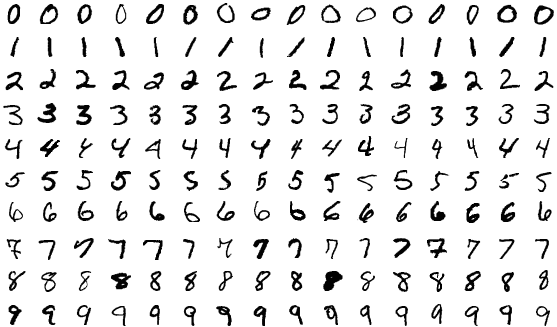
\includegraphics[width=0.8\textwidth]{informatica/ejemplo_mnist}
    \caption{Muestra de ejemplo de los dígitos del \textit{dataset} \textit{MNIST}. Imagen extraída de \cite{informatica:mnist_papers_with_code}}
\end{figure}


\subsection{Labeled Faces in the Wild}

La \textbf{segunda base de datos} con la que trabajamos es \textit{Labeled Faces in the Wild} (\textit{LFW}) \cite{informatica:lfw_dataset}. La base de datos se compone de algo más de 13.000 imágenes de caras extraídas de la web, en la que aparecen 5.749 individuos.

\begin{figure}[H]
    \centering
    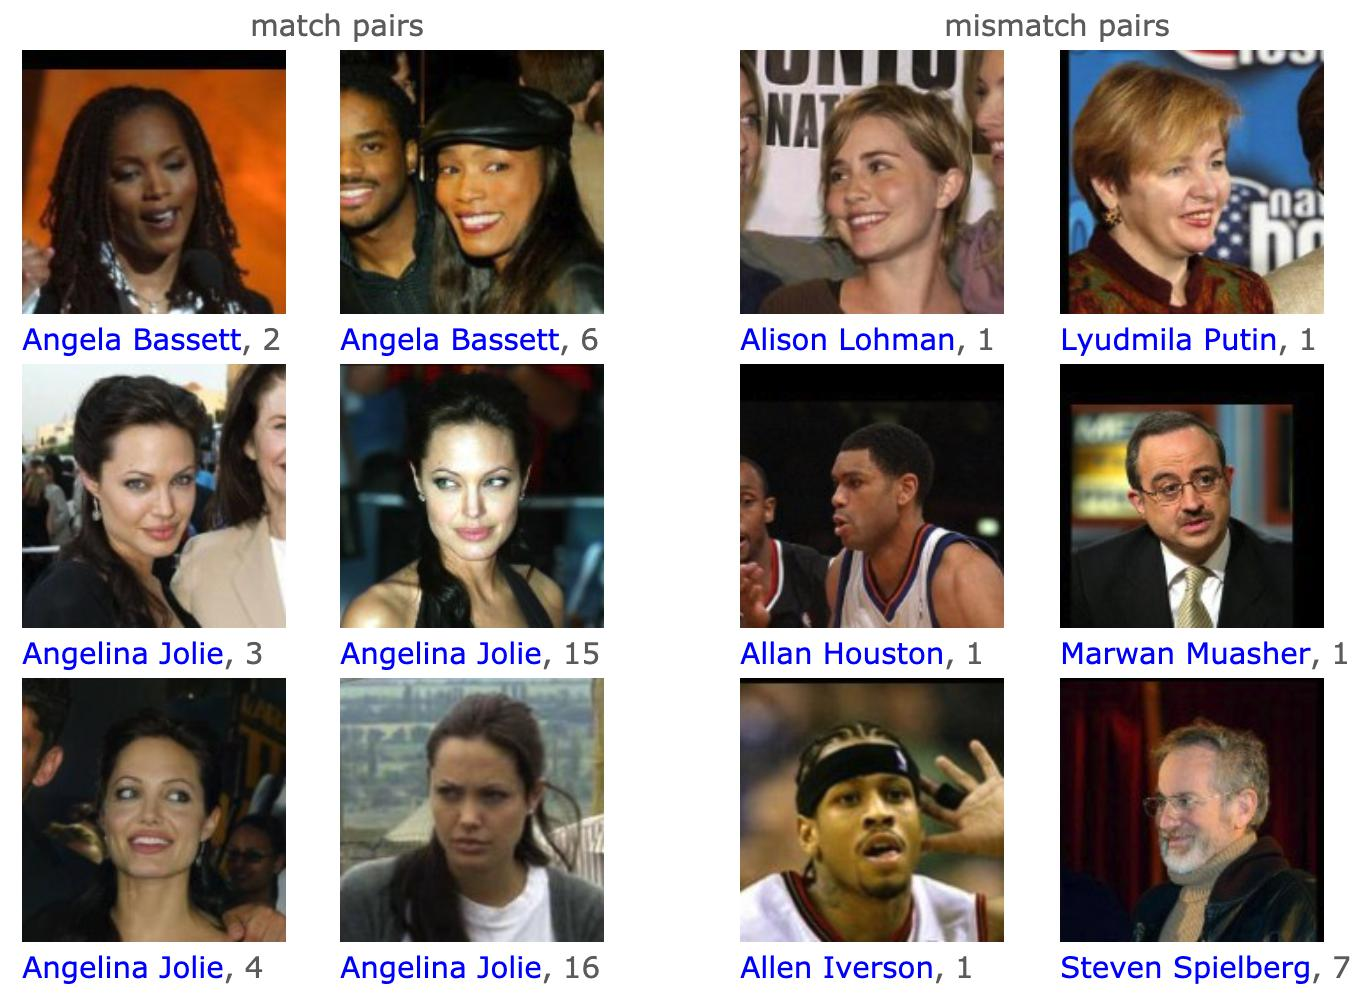
\includegraphics[width=0.8\textwidth]{informatica/ejemplo_lfw}
    \caption{Muestra de ejemplo del \textit{dataset} \textit{LFW}. Imagen extraída de \cite{informatica:papers_with_code_lfw}}
\end{figure}

En este caso damos un salto de calidad en cuanto a lo adecuada que es la base de datos a nuestro problema. Principalmente:

\begin{itemize}
    \item Estamos trabajando con imágenes faciales en vez de con imágenes de dígitos manuscritos
    \item El tamaño del \textit{dataset} ha aumentado considerablemente. Como veremos más adelante, en \sectionref{isec:optimizacion_codigo}, esto ya hace que tengamos que plantearnos optimizaciones de nuestros módulos de código
    \item La tarea de \textit{retrieval} ya tiene sentido (esto no ocurría al trabajar con dígitos manuscritos)
\end{itemize}

Tenemos una serie de \textbf{problemas con esta base de datos}, que motiva el uso de las dos últimas bases de datos:

\begin{itemize}
    \item En primer lugar, y como se indica en \cite{informatica:lfw_dataset}, esta base de datos está pensada para resolver una tarea de verificación. Aunque nos centremos en computar un \textit{embedding} (tarea que deberíamos poder resolver sin problemas), la propia institución ya nos está advirtiendo sobre lo inadecuada de la base de datos para intentar resolver una tarea de \textit{retrieval}
    \item Hay grupos que no están propiamente representados. Por ejemplo, apenas hay niños o personas por encima de los 80 años. Las mujeres y ciertos grupos étnicos están infrarrepresentados. En nuestro caso, es \textbf{especialmente grave la infrarrepresentación de ciertos grupos de edad}
    \item En \sectionref{ich:fundamentos_teoricos} hemos visto que para computar \textit{P-K batches} es fundamental que cada individuo tenga el máximo número de fotografías asociadas. De nada nos sirve, por ejemplo, tener una base de datos enorme pero con solo una fotografía por persona. En este sentido, y como indica \cite{informatica:lfw_dataset}, solo 1680 individuos tienen dos fotografías o más. Esto hace que tomar valores altos en el \textit{P-K sampling} sea imposible, y que por ello, tengamos que recurrir al aumentado de datos. Como comentaremos en \sectionref{isec:aumentado_datos}, esto será un reto importante de cara a mantener un rendimiento aceptable
    \item Este \textit{dataset} no introduce ninguna forma de trabajar la invarianza a cambios de edad, por lo que, en última instancia, no es adecuado para nuestros propósitos
\end{itemize}

\subsubsection{Distribución del número de imágenes por individuo} \label{isubsubs:imagenes_por_clase_lfw}

Acabamos de comentar la importancia de la distribución del número de imágenes por individuo. En la siguiente figura podemos observar dicha distribución:

\begin{figure}[H]
    \centering
    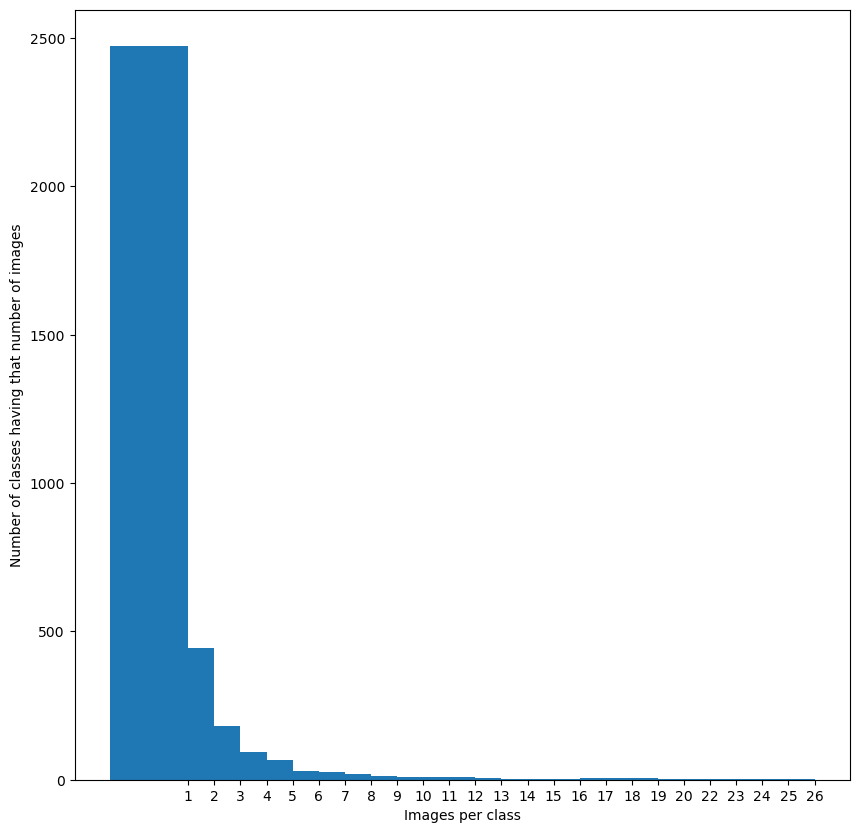
\includegraphics[width=0.6\textwidth]{informatica/lfw_images_per_class}
    \caption{Distribución del número de imágenes por cada individuo. En el eje horizontal, tenemos el número de imágenes por cada individuo. En vertical, la cantidad de individuos que tienen un cierto número de imágenes}
\end{figure}

Podemos ver que la mayoría de individuos solo tienen una imagen o dos. Teniendo en cuenta que casi siempre trabajamos usando al menos tres imágenes por clase, queda clara la necesidad de usar aumento de datos, que introduciremos en \sectionref{isec:aumentado_datos}.

Veamos cómo queda esta distribución tras forzar que cada individuo tenga al menos un número asociado de imágenes, usando aumentado de datos:

\begin{figure}[h!]
\centering
    \begin{subfigure}{0.5\textwidth}
        \centering
        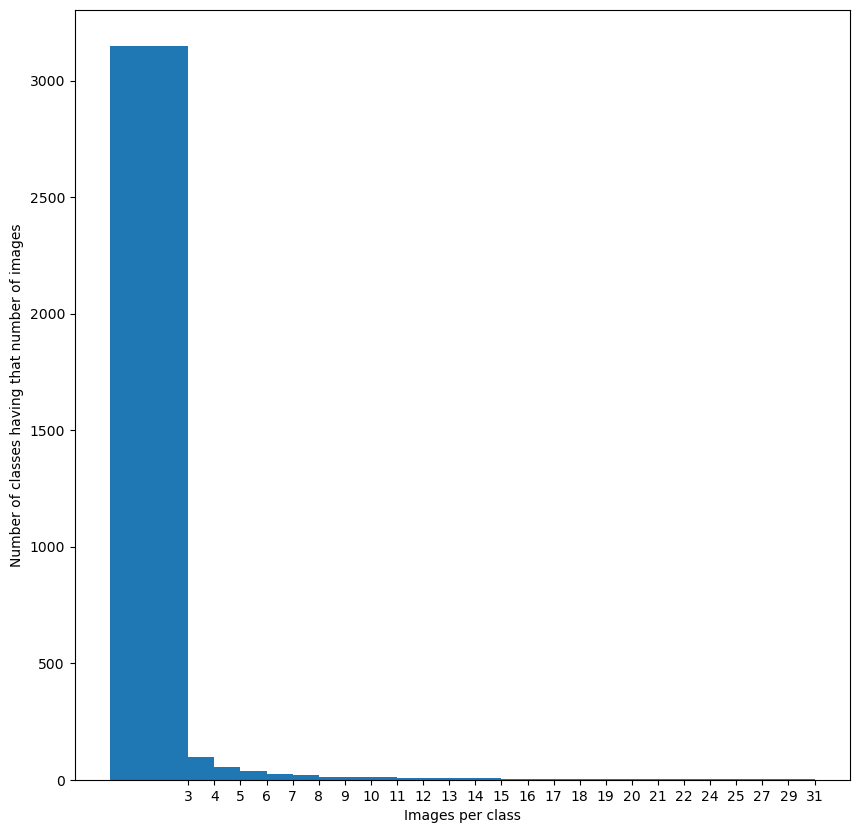
\includegraphics[width=.9\linewidth]{informatica/lfw_forzar_3}
        \caption{Forzando 3 imágenes por individuo }
    \end{subfigure}%
    \begin{subfigure}{.5\textwidth}
        \centering
        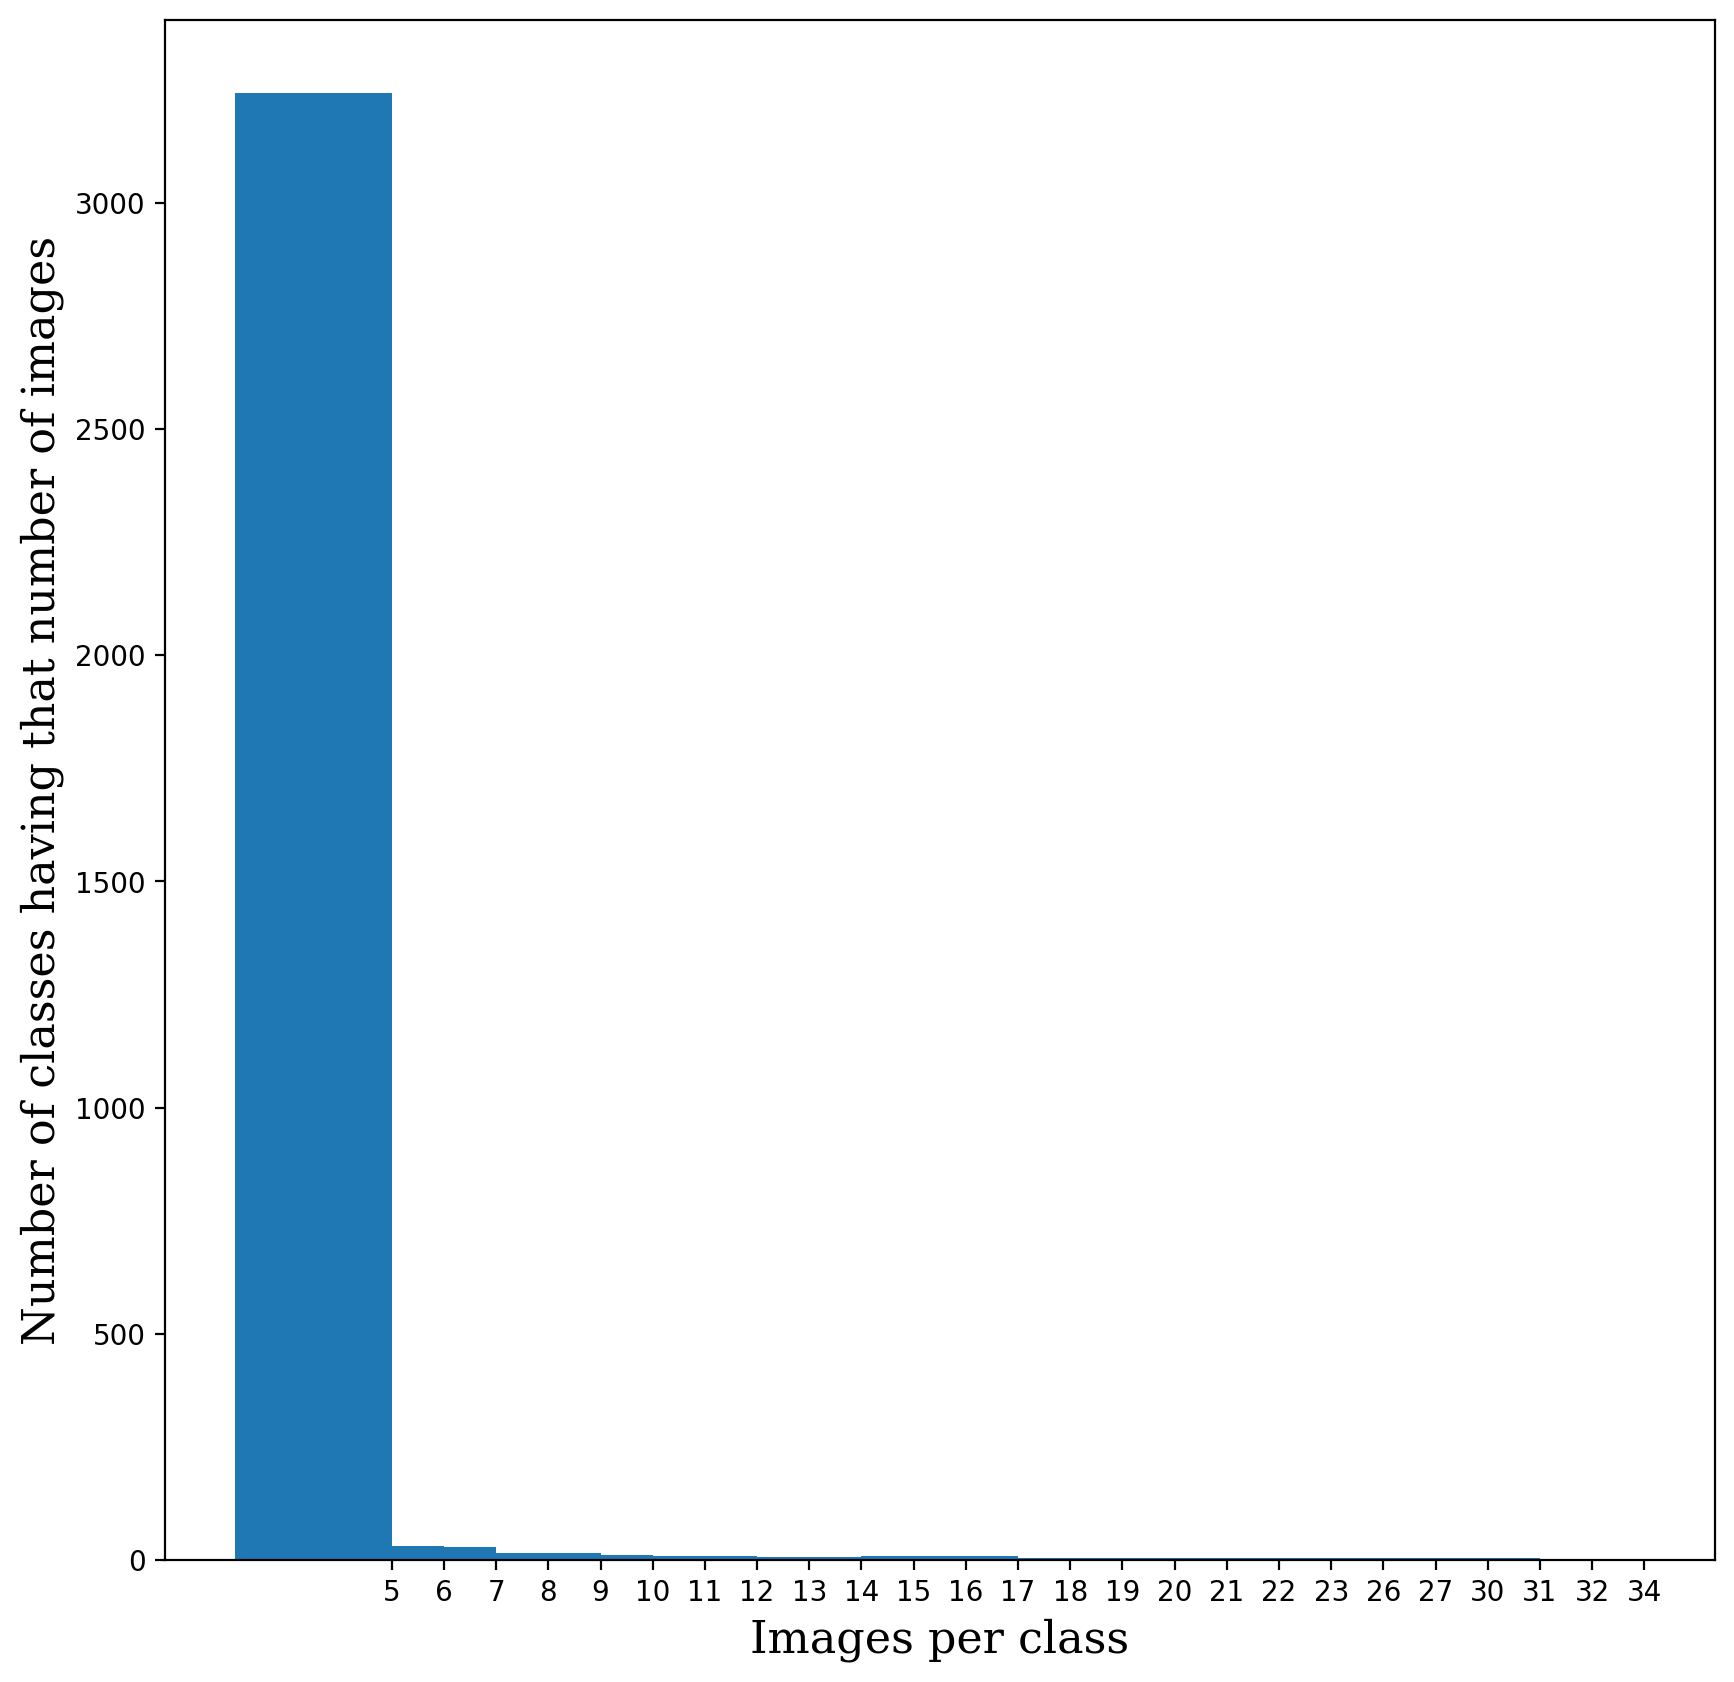
\includegraphics[width=.9\linewidth]{informatica/lfw_forzar_5}
        \caption{Forzando 5 imágenes por individuo}
    \end{subfigure}

    \begin{subfigure}{.5\textwidth}
        \centering
        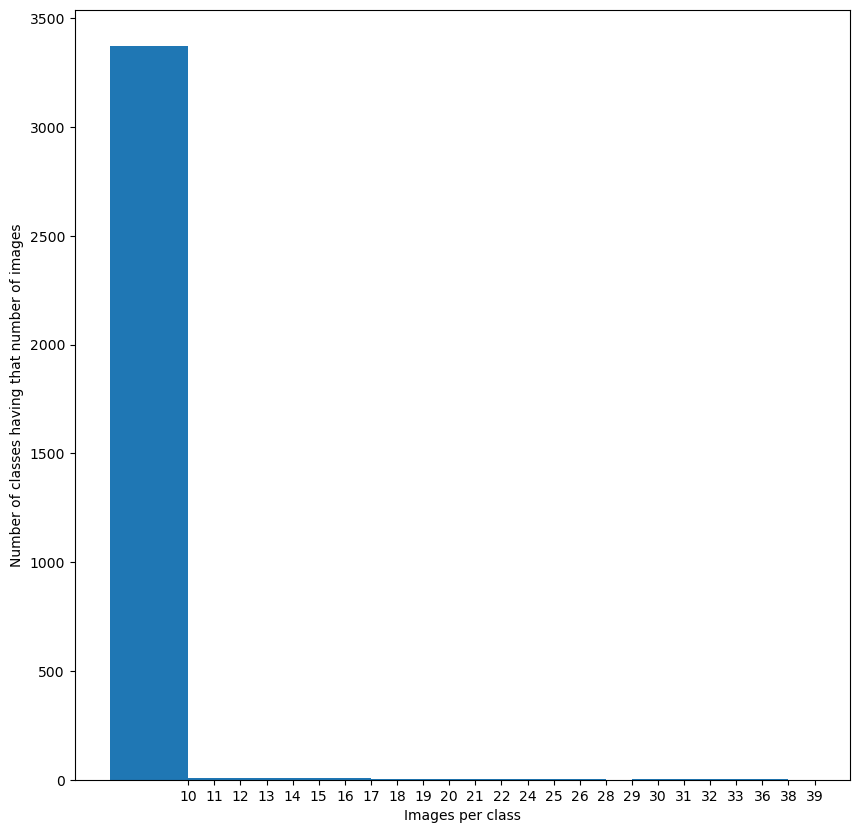
\includegraphics[width=.9\linewidth]{informatica/lfw_forzar_10}
        \caption{Forzando 10 imágenes por individuo }
    \end{subfigure}

    \caption{Distribuciones de imágenes por individuo tras aplicar \textit{data augmentation} para que cada clase tenga al menos $n$ individuos}
    \label{img:distribuciones_forzar_data_augmentation}
\end{figure}

Las distribuciones que se muestran en la \imgref{img:distribuciones_forzar_data_augmentation} muestran una propiedad clara: haciendo aumento de datos, la mayoría de individuos basan la variedad de sus imágenes en el aumento de datos. Además, esto ocurre por muy bajo que sea el número de imágenes por individuo que queramos obtener, como muestran las tres distribuciones prácticamente idénticas. Esto indica que seguramente los resultados obtenidos no vayan a ser demasiado buenos, puesto que la mayoría de imágenes de un individuo serán una o dos \entrecomillado{repetidas} (aunque apliquemos transformaciones propias del aumento de datos). Los posibles problemas que esto supone se agravan aún más al estar usando \textit{triplet loss} (véase \sectionref{isec:triplet_loss}).

Además, en este \textit{dataset} no tenemos información sobre las edades de los individuos en cada una de sus imágenes, así que no podemos hacer un estudio en más profundidad en este aspecto.

\subsection{\textit{FG-Net}} \label{isec:fgnet}

La \textbf{tercera base de datos} con la que trabajamos es \textit{FG-Net dataset}. La fuente original de este conjunto de datos ya no está operativa, y ahora estos datos se ofrecen en \cite{informatica:fgnet_dataset}. Este conjunto de datos se compone de 1.002 imágenes de 82 individuos distintos. Es el \textbf{\textit{dataset} más popular sobre \textit{AIFR}} \cite{informatica:best_fgnet_model}.

\begin{figure}[H]
    \centering
    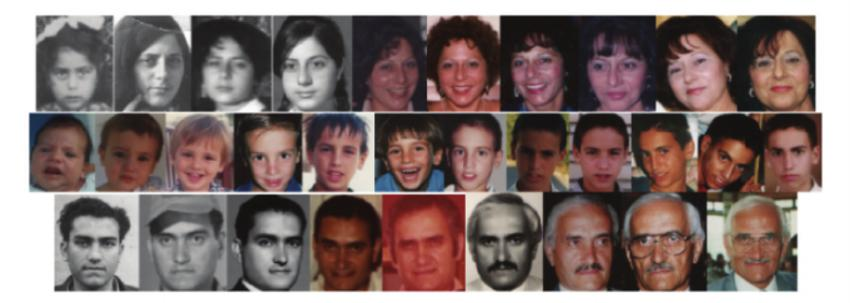
\includegraphics[width=0.8\textwidth]{informatica/ejemplo_fgnet}
    \caption{Muestra de ejemplo del \textit{dataset} \textit{FG-Net}. Imagen extraída de \cite{informatica:fg_net_papers_with_code}}
\end{figure}

Este conjunto de datos no se ofrece en ninguna librería conocida de \textit{machine learning}. Por tanto, y como indicamos posteriormente en \sectionref{isec:datasets_customs}, realizamos una implementación de \lstinline{torch.utils.data.Dataset} propia, para poder trabajar con estos datos.

Dicho conjunto de datos se compone de:

\begin{itemize}
    \item Un conjunto de imágenes. Los nombres de las imágenes deben ser procesados para extraer la identidad y edad de cada individuo
    \item Anotaciones de las imágenes. Estas anotaciones se componen de 68 puntos anotados por cada imagen
    \item Un archivo de \textit{Matlab} con 10 \textit{folds}, que el autor usa en \cite{informatica:yanweifu_work}
\end{itemize}

Optamos por trabajar únicamente con las imágenes, puesto que por las técnicas que estamos usando, no sabríamos aprovechar las anotaciones realizadas sobre los datos. Otros trabajos como \cite{informatica:facenet} usan esta forma de proceder. Gracias a los nombres de los archivos podemos almacenar también información sobre las edades de los individuos, información que va a ser muy relevante.

Y de nuevo, este \textit{dataset} presenta un salto de calidad respecto al anterior, por los siguientes motivos:

\begin{itemize}
    \item Trabajamos con un conjunto de datos cuya dificultad principal es la de la varianza en la edad. Esto se alinea por completo con el problema que queremos resolver
    \item El número de imágenes por individuo es mucho mejor que en \textit{LFW}, como muestran la \imgref{img:fgnet_images_per_class} y la \tableref{table:fgnet_images_per_class}
    \item Tenemos información sobre la distribución de la edad de nuestros individuos, que estudiamos en \sectionref{isubsubs:fgnet_dist_edades} y en \sectionref{isubsubs:fgnet_rango_edades}
\end{itemize}

\subsubsection{Distribución del número de imágenes por individuo}

A continuación, mostramos algunas características fundamentales del \textit{dataset}, empezando por la \textbf{distribución de número de imágenes por individuo}:

\begin{figure}[H]
    \centering
    \includegraphics[width=0.6\textwidth]{informatica/fgnet_images_per_class}
    \caption{Distribución del número de imágenes por cada individuo}
    \label{img:fgnet_images_per_class}
\end{figure}

Dicha distribución queda mejor explicada con las siguientes estadísticas:

\begin{table}[H]
\centering
\begin{tabular}{|l|l|}
    \hline
    \textbf{Estadística} & \textbf{Valor} \\
    \hline

    Media             & 12.22 \\
    Desviación típica & 2.15  \\
    Mínimo            & 6.00 \\
    Máximo            & 18.00 \\
    $Q1 \%$           & 11.00 \\
    $Q2 \%$           & 12.00 \\
    $Q3 \%$           & 13.00 \\

    \hline

\end{tabular}
\caption{Datos estadísticos sobre la distribución del número de imágenes por individuo}
\label{table:fgnet_images_per_class}
\end{table}

Tanto los estadísticos como la gráfica de la distribución dejan claro que, al menos en lo que respecta al número de imágenes por individuo, este conjunto de datos es mucho mejor. Como mínimo tenemos 6 imágenes por individuo, algo impensable en el conjunto de datos \textit{LFW}, donde apenas había individuos con más de dos imágenes. En segundo lugar, la media y los cuartiles nos muestran que la mayoría de los datos tienen entre 10 y 13 imágenes, lo que supone un muy buen dato.

\subsubsection{Distribución de edad de los individuos} \label{isubsubs:fgnet_dist_edades}

Veamos ahora la \textbf{distribución de la edad de los individuos}:

\begin{figure}[H]
    \centering
    \includegraphics[width=0.8\textwidth]{informatica/fgnet_distribucion_edades}
    \caption{Histograma de la variable edad en nuestro \textit{dataset}}
    \label{img:fgnet_histograma_edad}
\end{figure}

Que complementamos con las siguientes estadísticas

\begin{table}[H]
\centering
\begin{tabular}{|l|l|}
    \hline
    \textbf{Estadística} & \textbf{Valor} \\
    \hline

    Media  & 15.84 \\
    Mínimo & 0 \\
    Máximo & 69 \\
    Moda   & 18 \\

    \hline

\end{tabular}

    \caption{Algunas estadísticas sobre la distribución de la edad en nuestro conjunto de datos}
    \label{table:fgnet_estadisticas_edad}
\end{table}

El histograma dado en \imgref{img:fgnet_histograma_edad} nos muestra una distribución asimétrica, con una mayor concentración de individuos en edades bajas. Esto puede ser un problema a la hora de que un modelo entrenado sobre estos datos generalice adecuadamente. Por ejemplo, en el caso de que trabajemos con personas de una edad más adulta. En el histograma se observa un pico de frecuencia entorno a los 20 años. La moda nos indica que dicho pico se produce, en efecto, en los 18 años. Parece ser que dicha edad es un momento especial en el que se registran más fotografías de lo usual.

El rango de edades es muy amplio, yendo desde los 0 años (en \textit{LFW} ya comentábamos el problema que suponía no tener imágenes de niños) hasta los 69 años.

Es por esto que la calidad, en lo que distribución de edades se refiere, parece excelente. Aún así, podemos estudiar una distribución que nos dará una información todavía más profunda: el rango de edad por individuo.

\subsubsection{Distribución del rango de edad por individuo} \label{isubsubs:fgnet_rango_edades}

Estudiamos ahora el \textbf{rango de edad por individuo}. Para calcular este, computamos para cada individuo la diferencia entre su edad más avanzada menos su edad más temprana. Veamos este rango de edad gráficamente para todos los individuos:

\begin{figure}[H]
    \centering
    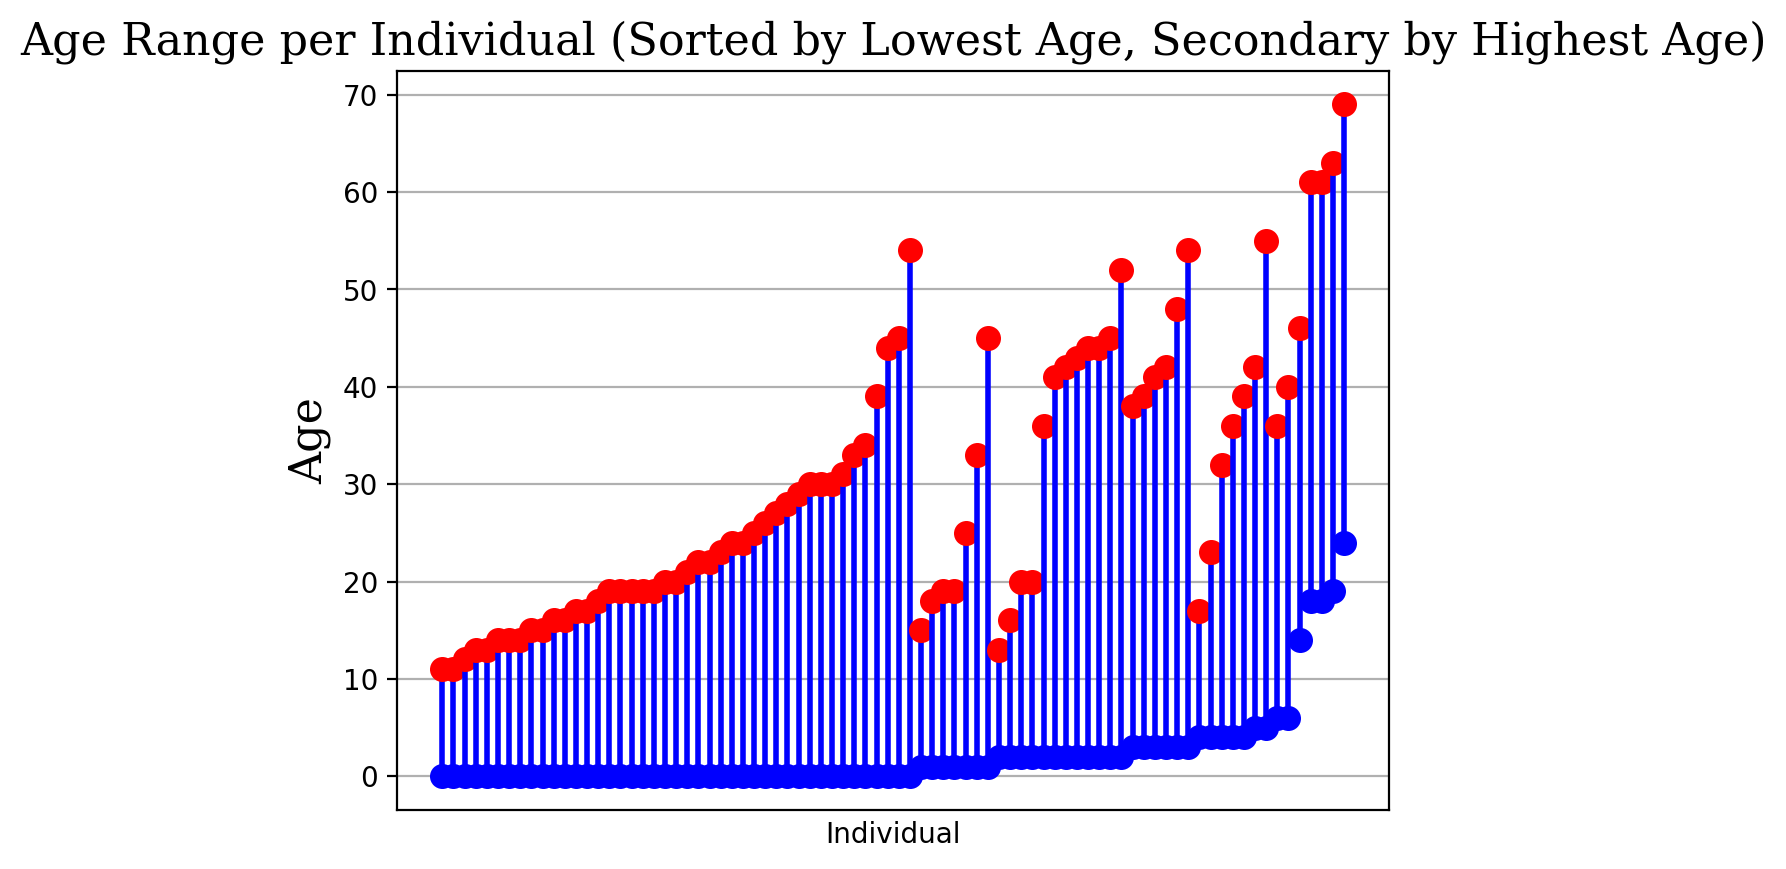
\includegraphics[width=0.8\textwidth]{informatica/fgnet_rangos_edad_individuales}
    \caption{Rangos de edad para todos los individuos. Los individuos están ordenados en primera instancia por su edad más baja, y en segunda instancia, por su edad más alta.}
    \label{img:fgnet_rangos_individuales}
\end{figure}

De esta forma es complicado sacar información de los datos. Así que mostremos la distribución de los rangos de edad en la \imgref{img:fgnet_rangos_distribucion}. Dicha distribución se complementa con los estadísticos de la \tableref{table:fgnet_rangos_estadisticas}:

\begin{figure}[h!]
    \centering
    \includegraphics[width=0.8\textwidth]{informatica/fgnet_distribucion_rangos_edad}
    \caption{Distribución del rango de edad. En el eje horizontal tenemos los rangos de edad. En el eje vertical, la cantidad de individuos que presentan dicho rango de edad en sus imágenes}
    \label{img:fgnet_rangos_distribucion}
\end{figure}

\begin{table}[h!]
\centering
\begin{tabular}{|l|l|}
    \hline
    \textbf{Estadística} & \textbf{Valor} \\
    \hline

    Media             & 27.80 \\
    Desviación Típica & 11.75 \\
    Mínimo            & 11.00 \\
    $Q_1 \%$          & 18.00 \\
    $Q_2 \%$          & 26.50 \\
    $Q_3 \%$          & 37.75 \\
    Máximo            & 55.00 \\

    \hline

\end{tabular}
\caption{Datos estadísticos sobre la distribución de los rangos de edad}
\label{table:fgnet_rangos_estadisticas}
\end{table}

En base a estos datos, podemos observar:

\begin{itemize}
    \item El rango mínimo de edad es de 11 años. Esto es, dado cualquier individuo del conjunto de datos, tenemos aseguradas imágenes que difieren en al menos 11 años. El máximo rango es de 55 años. Esto supone una gran riqueza en los datos, y a la vez, una gran dificultad a la hora de trabajar la invarianza a los cambios de edad
    \item De media tenemos un rango de aproximadamente 27 años. Y la mayoría de nuestros datos se encuentran dentro de unas diferencias de edad de entre 18 y 37 años (aproximadamente). De nuevo, esto marca la calidad en cuanto a rangos de edad se refiere
    \item En \imgref{img:fgnet_rangos_individuales} podemos ver claramente que la mayoría de individuos tienen imágenes en rangos de edad que podemos considerar bajos (por debajo de 10 años)
\end{itemize}

\subsubsection{Inconvenientes} \label{isubsubs:fgnet_inconvenientes}

Todo lo comentado previamente muestra los siguientes \textbf{inconvenientes}:

\begin{enumerate}
    \item Partimos de trabajar con únicamente 1.002 imágenes. Aunque lo hemos intentado, esta cantidad de datos no nos es suficiente para entrenar un modelo lo suficientemente potente de reconocimiento facial. Y mucho menos es suficiente para entrenar y además validar
    \item Como se comenta en \cite{informatica:best_fgnet_model}, este es el \textit{dataset} más famoso, pero a la vez, el más complicado de resolver en el ámbito de \textit{AIFR}. Esta complejidad ha quedado de sobra explicada en esta sección a través del estudio realizado, principalmente, sobre la distribución de edad y de rangos de edad
    \item Una forma de proceder común \cite{informatica:best_fgnet_model} es entrenar un modelo sobre un conjunto de datos mucho mayor, y usar \textit{FG-Net} únicamente para validar el modelo entrenado. Esta aproximación nos parece muy correcta por los siguientes motivos:
        \begin{itemize}
            \item En primer lugar, siempre es una buena idea comprobar que nuestro modelo generaliza correctamente, no solo sobre un subconjunto del \textit{dataset} original, sino sobre un conjunto de datos completamente nuevo
            \item En segundo lugar, hemos visto que la calidad de los datos en cuanto a rangos de edad es excelente, y supone un reto complejo. Por tanto, si obtenemos un modelo entrenado sobre otro conjunto de datos, que consigue un buen rendimiento en \textit{FG-Net}, podemos estar bastante seguros de que el modelo generalizará adecuadamente
            \item En tercer lugar, este proceso se asemeja bastante al uso que se le dará al modelo en la práctica, recibiendo imágenes de identidades nunca vistas con particularidades en el rango de edad que desconocemos a priori
        \end{itemize}
\end{enumerate}

Es por tanto que, siguiendo el procedimiento propuesto en \cite{informatica:best_fgnet_model}, usaremos este \textit{dataset} para validar el modelo entrenado sobre un conjunto de datos mucho mayor, en este caso, \sectionref{isec:dataset_cacd}.

\subsection{\textit{CACD}} \label{isec:dataset_cacd}

La \textbf{cuarta y última base de datos} con la que trabajamos es \entrecomillado{Cross-Age Celebrity Dataset} o \textit{CACD}. Como su propio nombre indica, se trata de una base de datos de celebridades en distintos momentos de su vida. Podemos acceder a estos datos en \cite{informatica:cacd_dataset}. El proceso de construcción de este conjunto de datos se especifica en \cite{informatica:paper_cacd}. En el momento de la publicación era el \textit{dataset} sobre \textit{AIFR} más grande.

Este \textit{dataset} se compone de 163.446 imágenes de 2.000 celebridades en edades que van desde los 16 hasta los 62 años \cite{informatica:paper_cacd}. Dichas imágenes fueron recolectadas de internet realizando búsquedas de ciertos individuos entre los años 2004 y 2013. Sabiendo la fecha de nacimiento de la celebridad, y el año de búsqueda, se computa la edad de dicha celebridad en cada imagen.

\begin{figure}[H]
    \centering
    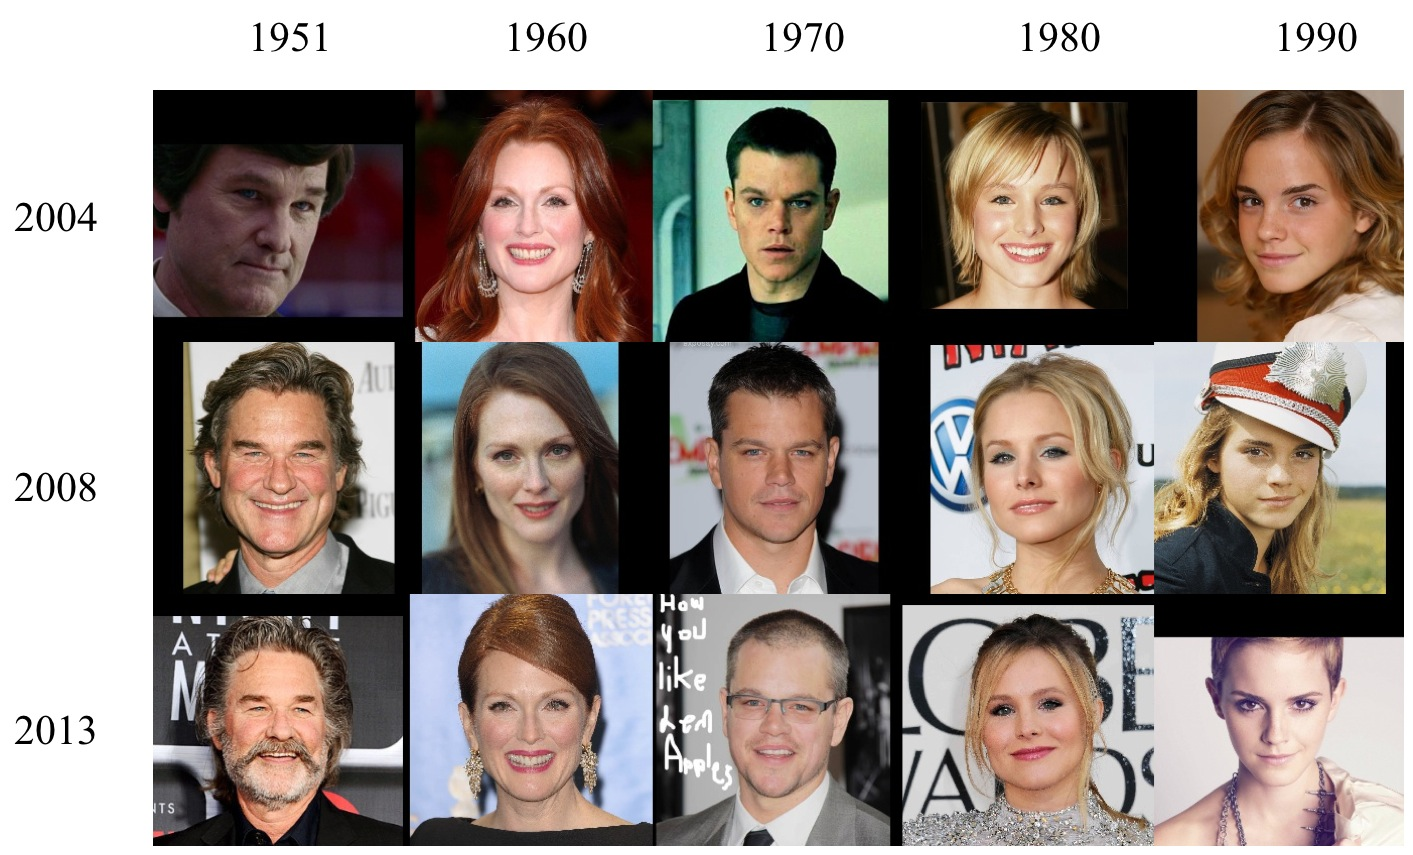
\includegraphics[width=0.8\textwidth]{informatica/cacd_example}
    \caption{Muestra de ejemplo del \textit{dataset} \textit{CACD}. En la parte superior, tenemos anotadas los años de nacimiento de los individuos. En la parte izquierda, tenemos anotados los años en los que las imágenes fueron tomadas. magen extraída de \cite{informatica:paper_cacd}}
    \label{img:cacd_imagenes_ejemplo}
\end{figure}

De nuevo, este conjunto de datos no se ofrece en ninguna librería conocida de \textit{machine learning}, por lo que realizamos otra implementación de \lstinline{torch.utils.data.Dataset}, como desarrollamos más adelante en \sectionref{isec:datasets_customs}. El conjunto de datos se compone de:

\begin{itemize}
    \item Las imágenes de las celebridades
    \item Información sobre las celebridades: nombre, identificador en la base de datos, año de nacimiento, posicionamiento en la página \url{IMBD.com}, y si la celebridad aparece o no en el \textit{dataset} \textit{LFW}
    \item Información sobre cada imagen: identificador de la celebridad, edad de la celebridad en la imagen, año en el que se tomó la imagen y \textit{landmarks} faciales
\end{itemize}

De nuevo, trabajamos únicamente con el conjunto de datos de imágenes, sin anotaciones (como se hace, por ejemplo, en \cite{informatica:facenet}). De los propios nombres de los archivos podemos extraer el identificador de la celebridad y la edad que tiene en cada una de sus imágenes. Este conjunto de datos mantiene algunas de las características que deseábamos y trae otras nuevas:

\begin{itemize}
    \item En primer lugar, tenemos varianza en la edad de los individuos, que es fundamental para resolver nuestro problema
    \item El tamaño del conjunto de datos ahora es elevado, con lo que podemos plantearnos el aprendizaje de un modelo lo suficientemente potente
    \item El número de imágenes por individuo es excelente, aún mejor que en \textit{FG-Net}, como mostraremos en \sectionref{isubsubs:cacd_images_per_indv}
\end{itemize}

Además, como hemos comentado en \sectionref{isubsubs:fgnet_inconvenientes}, usaremos este \textit{dataset} en conjunto con \textit{FG-Net}. Sobre este conjunto de datos se realizará principalmente el entrenamiento, usando \textit{FG-Net} únicamente para validar el modelo obtenido.

\subsubsection{Distribución del número de imágenes por individuo} \label{isubsubs:cacd_images_per_indv}

Veamos la \textbf{distribución del número de imágenes por cada individuo}:

\begin{figure}[H]
    \centering
    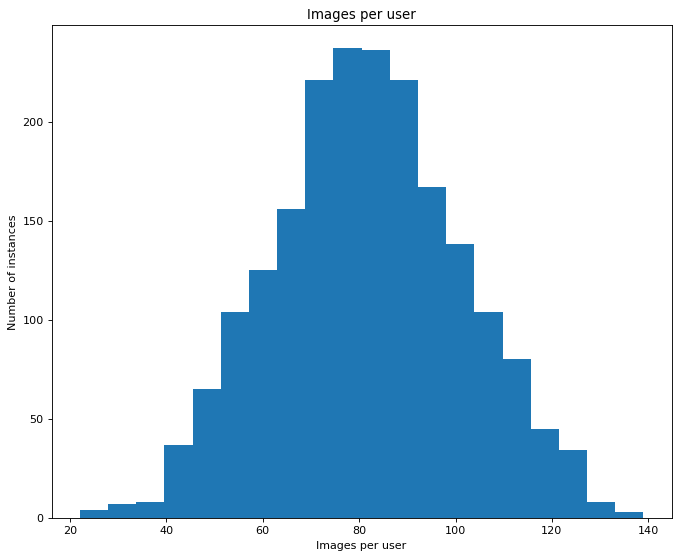
\includegraphics[width=0.7\textwidth]{informatica/cacd_images_per_class}
    \caption{Distribución del número de imágenes por cada individuo}
    \label{img:cacd_distr_images_per_class}
\end{figure}

De nuevo, complementamos con las siguientes estadísticas de la distribución:

\begin{table}[H]
\centering
\begin{tabular}{|l|l|}
    \hline
    \textbf{Estadística} & \textbf{Valor} \\
    \hline

    Media             & 81.72  \\
    Desviación típica & 19.51  \\
    Mínimo            & 22.00  \\
    $Q_1 \%$          & 68.00  \\
    $Q_2 \%$          & 81.00  \\
    $Q_3 \%$          & 95.00  \\
    Máximo            & 139.00 \\
    \hline

\end{tabular}
\caption{Datos estadísticos sobre la distribución del número de imágenes por individuo}
\end{table}

Podemos ver en la \imgref{img:cacd_distr_images_per_class}, que el número de imágenes por cada individuo parece seguir una distribución normal. Sin embargo, no nos interesa comprobar dicha hipótesis, pues es un hecho del que no vamos a aprovecharnos. Como mínimo, cada celebridad tiene 22 imágenes asociadas. Esto supone todavía una mejora respecto a \textit{FG-Net}. Llegamos a tener 139 imágenes por individuo como máximo. La mayoría de individuos tienen entre 68 y 95 imágenes asociadas. Por tanto, a la hora de establecer los valores del \textit{P-K sampling}, podemos tomar valores relativamente altos de $K$ (véase \sectionref{ich:fundamentos_teoricos}).

\subsubsection{Distribución de edad de los individuos}

Veamos ahora la \textbf{distribución de edad de los individuos}:

\begin{figure}[H]
    \centering
    \includegraphics[width=0.7\textwidth]{informatica/cacd_distribucion_edades}
    \caption{Histograma de la variable edad en nuestro \textit{dataset}}
\end{figure}

Complementamos con las siguientes estadísticas:

\begin{table}[H]
\centering
\begin{tabular}{|l|l|}
    \hline
    \textbf{Estadística} & \textbf{Valor} \\
    \hline

    Media  & 38.03 \\
    Mínimo & 14    \\
    Máximo & 62    \\
    Moda   & 37    \\

    \hline

\end{tabular}
\caption{Algunas estadísticas sobre la distribución de la edad en nuestro conjunto de datos}
\end{table}

Esta vez tenemos una distribución más simétrica de las edades, con una media de aproximadamente 38 años. La edad mínima es de 14 años, muy alejada de los 0 años de \textit{FG-Net} (\tableref{table:fgnet_estadisticas_edad}). Esto puede suponer algunos problemas a la hora de entrenar un modelo en \textit{CACD} y que generalice correctamente en \textit{FG-Net}. No entraremos en comparaciones más profundas, pues esto lo haremos en \sectionref{isec:comparaciones_datasets}.

\subsubsection{Distribución del rango de edad por individuo}

Veamos ahora los \textbf{rangos de edad} de cada uno de los individuos del conjunto de datos:

\begin{figure}[H]
    \centering
    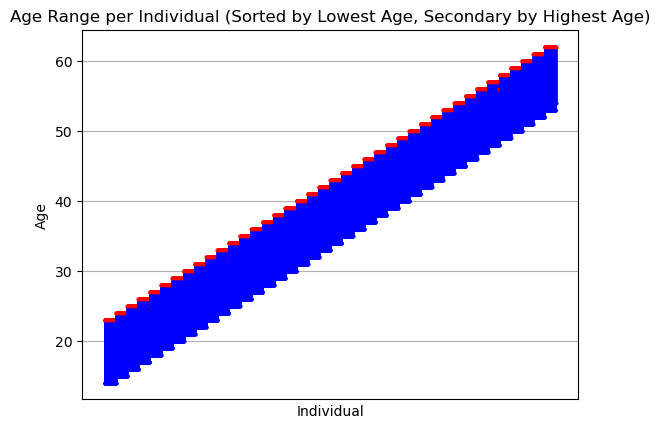
\includegraphics[width=0.6\textwidth]{informatica/cacd_rangos_individuales}
    \caption{Rangos de edad para todos los individuos. Los individuos están ordenados en primera instancia por su edad más baja, y en segunda instancia, por su edad más alta.}
\end{figure}

Esta gráfica ahora no es tan clara como cuando la presentábamos para \textit{FG-Net} en la \imgref{img:fgnet_rangos_distribucion}, así que procedemos a hacer algunas observaciones. En primer lugar, como se han recolectado los datos buscando imágenes correspondientes al periodo 2004-2013, el rango de edad siempre va a ser de 9 años. Esto lo vamos a comprobar posteriormente. Por esto mismo, y por el ordenamiento en base a la edad más baja de cada individuo, estamos visualizando la distribución de las edades. Es decir, fijándonos en el punto más bajo de cada línea, estamos viendo a aquellos individuos que en 2004 tenían cierta edad. Así que se pueden visualizar, de una forma poco conveniente, los grupos de edad presentes en nuestra base de datos.

Confirmemos esto viendo las estadísticas sobre la distribución de los rangos de edad:

\begin{table}[H]
\centering
\begin{tabular}{|l|l|l|l|}
    \hline
    \textbf{Estadística} & \textbf{Valor} \\
    \hline

    Media             & 8.99 \\
    Desviación típica & 0.11 \\
    Mínimo            & 7.00 \\
    $Q_1 \%$          & 9.00 \\
    $Q_2 \%$          & 9.00 \\
    $Q_3 \%$          & 9.00 \\
    Máximo            & 9.00 \\

    \hline

\end{tabular}
    \caption{Datos estadísticos sobre la distribución de los rangos de edad}
\end{table}

Vemos que prácticamente todos los individuos tienen un rango de edad de nueve años. Podemos ver que tenemos un valor mínimo de 7 años. Por tanto, sabemos que tenemos algunos casos de individuos que no tienen cierta banda inicial o final de edades. Esto puede deberse a defunciones antes del 2013, o que el individuo era muy joven y no se disponían de imágenes suyas alrededor de 2004. Realizando una simple consulta sobre la base de datos, vemos que únicamente 15 individuos, de los 2000 individuos que componen la base de datos, tienen un rango de edad distinto a 9 años. Esto hace que sea completamente insignificativo.

Por tanto, es totalmente innecesario mostrar el histograma de los rangos de edad.

\subsubsection{Inconvenientes}

Todo esto plantea los siguientes \textbf{inconvenientes}:

\begin{itemize}
    \item En primer lugar, los rangos de edad son muy pequeños y nada variables. Por ejemplo, en \imgref{img:cacd_imagenes_ejemplo} podemos observar algunos casos en los que hay poca variabilidad por el paso de los años. Además, nuestro modelo siempre va a trabajar con diferencias de como mucho 9 años. No sabemos cómo puede comportarse cuando trabajemos con otros rangos de edad
    \item En segundo lugar, y como comentaremos detalladamente en \sectionref{isec:comparaciones_datasets}, el conjunto de entrenamiento y de validación son muy distintos. Por ejemplo, no tenemos imágenes de personas por debajo de 14 años en \textit{CACD}, mientras que en \textit{FG-Net} hemos visto que tenemos imágenes desde cero años.
    \item Por tanto, es realmente complicado que el modelo generalice. Sin embargo, de ser así, estaremos bastante seguros de haber construido un modelo robusto
\end{itemize}

\subsection{Comparación de los \textit{datasets} \textit{FG-Net} y \textit{CACD}} \label{isec:comparaciones_datasets}

Como hemos comentado, tanto en \sectionref{isec:fgnet} como en \sectionref{isec:dataset_cacd}, usaremos el primer \textit{dataset} para entrenar nuestro modelo, y el segundo para validar los resultados obtenidos. Por tanto, es relevante realizar una comparación de ciertas propiedades de ambos conjuntos de datos. Repasaremos los apartados de estudio realizados en los dos últimos \textit{datasets}, comparando los resultados de ambos.


\subsubsection{Distribución del número de imágenes por individuo}

\begin{figure}[H]
\centering
    \begin{subfigure}{.5\textwidth}
        \centering
        \includegraphics[width=0.95\linewidth]{informatica/fgnet_images_per_class}
        \caption{\textit{FG-Net}}
    \end{subfigure}%
    \begin{subfigure}{.5\textwidth}
        \centering
        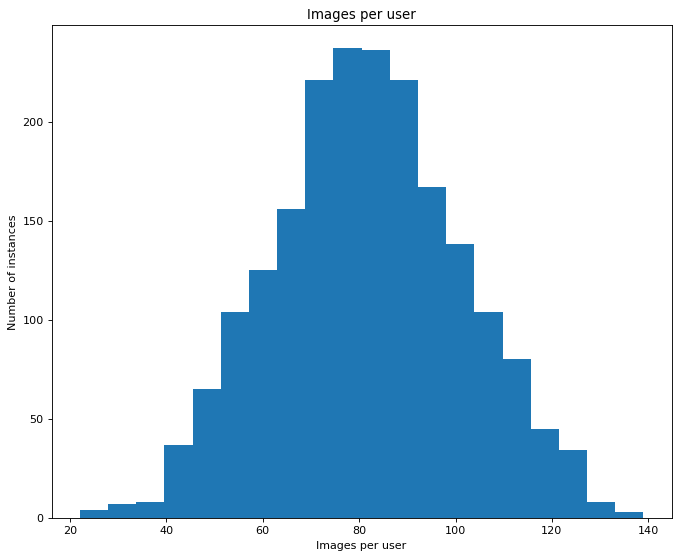
\includegraphics[width=0.95\linewidth]{informatica/cacd_images_per_class}
        \caption{\textit{CACD}}
    \end{subfigure}
\caption{Distribución del número de imágenes por individuo en los \textit{datsets} \textit{FG-Net} y \textit{CACD} }
    \label{img:comparativa_imagenes_por_individuo}
\end{figure}


\begin{table}[H]
\centering
\begin{tabular}{|l|l|l|}
    \hline
    \textbf{\textit{Estadística}} & \textbf{\textit{FG-Net}} & \textbf{\textit{CACD}} \\
    \hline

    Media             & 12.22 & 81.72  \\
    Desviación típica & 2.15  & 19.51  \\
    Mínimo            & 6.00  & 22.00  \\
    Máximo            & 18.00 & 68.00  \\
    $Q1 \%$           & 11.00 & 81.00  \\
    $Q2 \%$           & 12.00 & 95.00  \\
    $Q3 \%$           & 13.00 & 139.00 \\

    \hline

\end{tabular}
\caption{Datos estadísticos sobre la distribución del número de imágenes por individuo, en los \textit{datasets} \textit{FG-Net} y \textit{CACD}}
    \label{table:comparativa_imagenes_por_individuo}
\end{table}

En base a los datos mostrados en \imgref{img:comparativa_imagenes_por_individuo} y \tableref{table:comparativa_imagenes_por_individuo}, podemos ver que:

\begin{itemize}
    \item El número de imágenes por individuo es ampliamente superior en \textit{CACD} que en \textit{FG-Net}. Un claro indicador de esto es que el valor máximo en \textit{FG-Net} está por debajo del mínimo en \textit{CACD}. Este hecho puede ayudar a solventar algunos de los problemas sobre la diferencia en la distribución de la edad que plantea \textit{FG-Net}
    \item La desviación típica es mucho menor en \textit{FG-Net}. Por lo tanto, respecto al número de imágenes por individuo, quizás \textit{CACD} suponga algo más de dificultad, aunque esto no nos parece un factor realmente relevante
    \item A la hora de entrenar, vamos a poder usar valores mucho más altos de $K$ en \textit{CACD} (véase \sectionref{isubs:muestreo_datos_pk_sampling_teoria}). Y este valor, en validación, se puede reducir (o directamente ignorar) para actuar sobre \textit{FG-Net}
    \item La distribución en \textit{CACD} parece seguir una distribución normal, mientras que en \textit{FG-Net}, a priori, no se ve de forma tan clara. Aunque como ya hemos comentado previamente, no estamos interesados en comprobar estas hipótesis
\end{itemize}

\subsubsection{Distribución de edad de los individuos} \label{isubsubs:conjunta_fgnet_cacd_edades}

\begin{figure}[H]
\centering
    \begin{subfigure}{.5\textwidth}
        \centering
        \includegraphics[width=0.95\linewidth]{informatica/fgnet_distribucion_edades}
        \caption{\textit{FG-Net}}
    \end{subfigure}%
    \begin{subfigure}{.5\textwidth}
        \centering
        \includegraphics[width=0.95\linewidth]{informatica/cacd_distribucion_edades}
        \caption{\textit{CACD}}
    \end{subfigure}
    \caption{Distribuciones de las edades en los \textit{datasets} \textit{FG-Net} y \textit{CACD}}
    \label{img:conjunta_fgnet_cacd_edades}
\end{figure}

\begin{table}[H]
\centering
\begin{tabular}{|l|l|l|}
    \hline
    \textbf{Estadística} & \textbf{\textit{FG-Net}} & \textbf{\textit{CACD}} \\
    \hline

    Media  & 15.84 & 38.03 \\
    Mínimo & 0     & 14    \\
    Máximo & 69    & 62    \\
    Moda   & 18    & 37    \\

    \hline

\end{tabular}
    \caption{Estadísticas sobre la distribución de la edad en los \textit{datasets} \textit{FG-Net} y \textit{CACD}}
    \label{table:conjunta_fgnet_cacd_estadisticas_edad}
\end{table}

A partir de estos datos, podemos ver que:

\begin{itemize}
    \item Las formas de las dos distribuciones de datos, tal y como se aprecia en \imgref{img:conjunta_fgnet_cacd_edades}, son completamente distintas. Por un lado, en \textit{FG-Net} tenemos una distribución muy asimétrica, acumulando la mayor parte de la densidad en edades bajas, entre 0 y 20 años. En \textit{CACD}, tenemos una distribución más o menos simétrica
    \item El dominio en \textit{FG-Net} es mucho más amplio, con una edad mínima 14 años menor, y una edad máxima 7 años mayor
    \item Por tanto, era razonable pensar que íbamos a tener una población mucho más adulta en \textit{CACD}, como muestran tanto los histogramas como el valor de la media y moda en \tableref{table:conjunta_fgnet_cacd_estadisticas_edad}
    \item La concentración en edades bajas en \textit{FG-Net} puede presentar un \textbf{serio problema} a la hora de que un modelo entrenado sobre \textit{CACD} funcione correctamente
\end{itemize}

\subsubsection{Distribución del rango de edad por individuo}

\begin{figure}[H]
    \centering
    \begin{subfigure}[t]{0.55\textwidth}
        \centering
        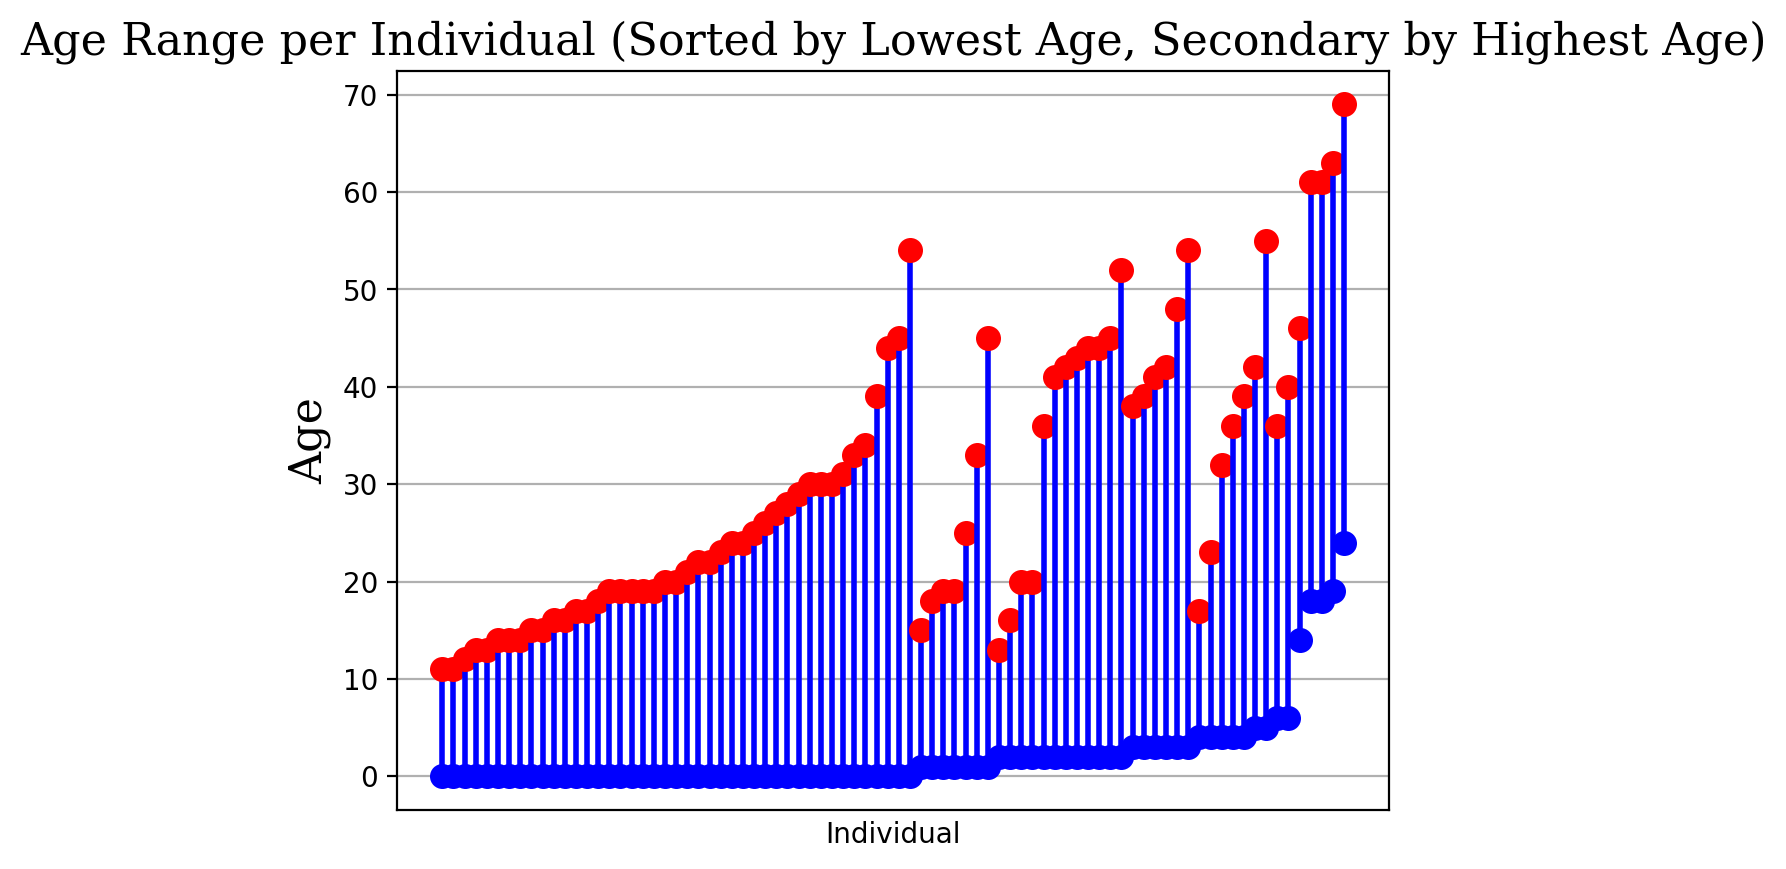
\includegraphics[width=0.95\linewidth]{informatica/fgnet_rangos_edad_individuales}
        \caption{\textit{FG-Net}}
    \end{subfigure}
    \begin{subfigure}[t]{0.4\textwidth}
        \centering
        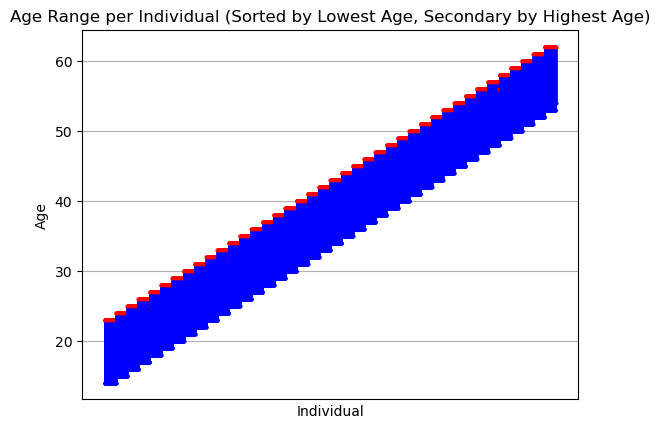
\includegraphics[width=0.95\linewidth]{informatica/cacd_rangos_individuales}
        \caption{\textit{CACD}}
    \end{subfigure}

    \caption{Rangos de edad para todos los individuos, en los \textit{datasets} \textit{FG-Net} y \textit{CACD}. Los individuos están ordenados en primera instancia por su edad más baja, y en segunda instancia, por su edad más alta.}
    \label{img:conjunta_fgnet_rangos_edades_individuales}
\end{figure}

\begin{table}[H]
\centering
\begin{tabular}{|l|l|l|}
    \hline
    \textbf{Estadística} & \textbf{\textit{FG-Net}} & \textbf{\textit{CACD}} \\
    \hline

    Media             & 27.80 & 8.99 \\
    Desviación Típica & 11.75 & 0.11 \\
    Mínimo            & 11.00 & 7.00 \\
    $Q_1 \%$          & 18.00 & 9.00 \\
    $Q_2 \%$          & 26.50 & 9.00 \\
    $Q_3 \%$          & 37.75 & 9.00 \\
    Máximo            & 55.00 & 9.00 \\

    \hline

\end{tabular}
\caption{Datos estadísticos sobre la distribución de los rangos de edad, para los \textit{datasets} \textit{FG-Net} y \textit{CACD}}
    \label{table:conjunta_fgnet_estadisticas_rangos_edad}
\end{table}

A partir de esto, podemos ver que:

\begin{itemize}
    \item Como muestran tanto la \imgref{img:conjunta_fgnet_rangos_edades_individuales} como la \tableref{table:conjunta_fgnet_estadisticas_rangos_edad}, \textit{FG-Net} presenta una variabilidad en los rangos de edad que es prácticamente inexistente en \textit{CACD} (en la que salvo 15 individuos, el rango de edad siempre es de 9 años)
    \item Este problema se ve agravado cuando nos damos cuenta que la mayoría de individuos en \textit{FG-Net} tienen un rango de edad entre 18 y casi 38 años, que contrasta con el rango de 9 años constante en \textit{CACD}. Si el rango en \textit{CACD} fuese constante pero superior, al menos la falta de variabilidad podría no notarse tanto
    \item Para \textit{FG-Net} tenía sentido mostrar el histograma de la distribución de rangos, en \imgref{img:fgnet_rangos_distribucion}. Sin embargo, en \textit{CACD}, como no teníamos variabilidad, no mostramos dicho histograma
    \item Así que las dificultades que veíamos en \sectionref{isubsubs:conjunta_fgnet_cacd_edades} se ven agravadas al estudiar la distribución de los rangos de edad
\end{itemize}

\section{Entorno de ejecución} \label{isec:entorno_ejecucion}

Durante la implementación del código y el proceso de experimentación, hemos trabajado en tres \textbf{entornos de desarrollo y ejecución} distintos:

\begin{enumerate}
    \item El entorno de \textbf{desarrollo local}, nuestro ordenador portátil. Lo hemos usado principalmente para implementar el código y ejecutar algunos \textit{tests}. Por su baja potencia, no lo hemos usado ni para lanzar los \textit{Notebooks} de \textit{Jupyter} sobre los que realizamos la exploración de datos, ni para lanzar los \textit{scripts} de aprendizaje. Por tanto, no resulta interesante mostrar sus especificaciones

    \item En fases tempranas del proyecto hemos escrito y ejecutado código en \textbf{\textit{Google Colab}}. Esta plataforma nos permite ejecutar, a través de una interfaz \textit{web}, \textit{Notebooks} de \lstinline{Python}.

        \begin{itemize}
            \item Además, otorga de forma limitada algunos recursos como acceso a cómputo \textit{TPU}. Las \textit{Tensor Processing Units} o \textit{TPUs} son tecnología \textit{hardware} propietaria de \textit{Google}, que busca optimizar el entrenamiento e inferencia de modelos de IA \cite{informatica:google_tpu}.

            \item Los \textit{Notebooks} en \textit{Google Colab} vienen con la mayoría de bibliotecas de aprendizaje automático pre-instaladas. Esto es una gran ventaja al inicio del desarrollo, puesto que evitamos enfrentarnos a la complejidad de configurar un entorno de ejecución \lstinline{Python}

            \item Sin embargo, rápidamente tenemos que abandonar este entorno por dos motivos: el acceso a recursos es demasiado limitado, y solo poder usar código escrito en \textit{Notebooks} es una restricción importante.

            \item El \textit{hardware} que se pone a disposición del usuario se asigna dinámicamente, en base al consumo previo de recursos del usuario y a la demanda actual. Por tanto, no podemos obtener una especificación estática de los recursos de los que disponemos \cite{informatica:google_colab_faq}. Tampoco existe documentación oficial donde se especifique qué \textit{hardware} se ofrece, cuotas de consumo, \ldots\; Sin embargo, accediendo a un \textit{Notebook}, podemos ejecutar algunos comandos para ver los recursos que nos ofrecen en un momento dado \footnote{Dichos comandos son ejecutados el 18 de Septiembre de 2023}

                \begin{itemize}
                    \item El comando \lstinline{df -h} nos muestra que tenemos disponibles 50GB de memoria permanente. Sin embargo, esto no es una limitación porque podemos conectar nuestra cuenta de usuario de \textit{Google} para acceder a todos los datos almacenados en \textit{Google Drive}
                    \item El comando \lstinline{cat /proc/cpuinfo} nos muestra que estamos usando una \textit{CPU} \entrecomillado{Intel ( R ) Xeon ( R ) @ 2.20 GHz}
                    \item El comando \lstinline{cat /proc/meminfo} nos muestra que disponemos de aproximadamente 12GB de memoria \textit{RAM}
                    \item Sabemos que podemos acceder a \textit{TPUs} de \textit{Google}, pero no disponemos de ningún comando para acceder a las especificaciones de este \textit{hardware}
                \end{itemize}
        \end{itemize}

    \item Los \textbf{servidores clúster GPU de la Universidad de Granada, \textit{nGPU}}.
        \begin{itemize}
            \item Estos servidores se encuentran en el Centro de Procesado de Datos (\textit{CPD}) Santa Lucía. Para trabajar con estos servidores, accedemos por \lstinline{ssh} a un nodo cabecera, y usando el programa \lstinline{slurm}, enviamos trabajos a los distintos nodos que componen el \textit{CPD}.
            \item Hemos usado estos servidores tanto para lanzar \textit{Notebooks} en los que realizamos principalmente análisis exploratorio de datos, como para lanzar \textit{scripts} de \lstinline{Python} usados principalmente para llevar a cabo el entrenamiento y validación de modelos
            \item El \textit{hardware} de los nodos \textit{Titan} y \textit{Atenea}, los dos nodos que hemos usado mayoritariamente, es el siguiente:
                \begin{itemize}
                    \item Dos procesadores \textit{Intel® Xeon® E5-2630}, cada uno
                    \item Memoria \textit{RAM} \textit{DDR4} de 128 GB
                    \item Memoria permantente de 2,7TB
                    \item El nodo \textit{Titan} dispone de tres \textit{GPUs} \textit{GTX Titan X Pascal} y una \textit{GPU} \textit{GTX Titan Xp}, mientras que el nodo \textit{Atenea} dispone de cuatro \textit{GPUs} \textit{GTX Titan Xp}
                \end{itemize}
        \end{itemize}

\end{enumerate}

Como \textbf{lenguaje de programación} usaremos \lstinline{Python}, en su versión 3.10.2. Para la \textbf{gestión de entornos} de \lstinline{Python} usaremos dos tecnologías:

\begin{enumerate}
    \item El gestor de paquetes y entornos \textbf{\lstinline{Conda}} \cite{informatica:conda_web}. Este gestor nos permite instalar fácilmente paquetes de \lstinline{Python} en entornos virtuales, evitando así instalarlos a nivel de sistema (lo que puede provocar conflictos con versiones de paquetes usados en otros proyectos). Además, permite generar un archivo \lstinline{enviroment.yml} que especifica exactamente qué paquetes están instalados y con qué versión. A partir de dicho fichero podremos reproducir el entorno de desarrollo en diferentes máquinas. Por ejemplo, tenemos el mismo entorno de desarrollo en nuestro ordenador portátil y en los servidores donde se ejecutan los entrenamientos. Junto con el uso de contenedores \lstinline{docker} (enfoque que consideramos muy complejo), es la única alternativa que tenemos para configurar nuestro entorno de desarrollo en los servidores \textit{nGPU}
    \item \textbf{\lstinline{nix}} \cite{informatica:nixos_web}. Dicha tecnología se compone de un lenguaje funcional puro, que se usa en su gestor de paquetes reproducible y declarativo. Usamos esta tecnología en nuestro ordenador por su robustez: durante los meses de desarrollo, algunas librerías se rompen en sus últimas versiones. Con \lstinline{nix} podemos volver cómodamente a versiones previas de todo el entorno de desarollo (\entrecomillado{rollback}). Esto se puede conseguir también con \lstinline{Conda} pero es mucho más complicado. Además, permite especificar paquetes de \lstinline{Python}, paquetes de \textit{Latex} usados para producir esta memoria y paquetes de \textit{Linux}. Es decir, no se limita únicamente a gestionar entornos de \lstinline{Python}
\end{enumerate}

Como \textbf{sistema operativo}, hemos usado:

\begin{itemize}
    \item En nuestro entorno de desarrollo, la distribución de \textit{Linux} \textit{NixOS} en su versión 23.11
    \item En \textit{Google Colab}, la distribución de \textit{Linux} \textit{Ubuntu} en su versión 22.04.2 \textit{LTS} \footnote{Comprobamos esta versión ejecutando el comando \lstinline{lsb_release -d} el 19 de Septiembre de 2023}
    \item En los servidores \textit{nGPU}, la distribución de \textit{Linux} \textit{Ubuntu} en su versión 20.04.5 \textit{LTS}
\end{itemize}

\section{Técnicas empleadas}

A continuación, presentamos diversas técnicas que hemos empleado en nuestro trabajo. Estas técnicas abarcan aspectos muy diversos: en \sectionref{isec:hptuning_kfold_cross_validation} introducimos una técnica que forma parte del diseño experimental, en \sectionref{isubs:normalizacion_teoria} presentamos una técnica que forma parte del diseño de la solución y finalmente, en \sectionref{isubs:localizacion_partes_criticas} describimos una técnica fundamental para optimizar nuestra base de código.

Aunque pertenezcan a ambientes muy diferentes, incluimos estas técnicas aquí, ya que resultarán fundamentales si el lector decide explorar el capítulo \sectionref{ich:implementacion}, en cuyo caso será crucial comprender estos métodos dado que en dicha sección estudiamos detalladamente su implementación.

\subsection{Hyperparameter Tuning} \label{isec:hptuning_kfold_cross_validation}

Como veremos más adelante, a la hora de realizar un entrenamiento para producir un modelo que resuelva nuestra tarea, hemos de \textbf{fijar una serie de hiperparámetros} que afectan de forma esencial a la calidad de dicho modelo. Algunos hiperparámetros son la tasa de aprendizaje o \textit{learning rate}, la dimensión del \textit{embedding} semántico que aprende nuestro modelo, el valor de $\{P, K\}$ (véase \sectionref{isubs:muestreo_datos_pk_sampling_teoria}), el número de épocas de entrenamiento, ... Buscamos por tanto técnicas que nos permitan decidir el valor de los hiperparámetros en base a los datos de los que disponemos.

Una técnica de \textbf{\textit{hyperparameter tuning}} estará formada por dos componentes:

\begin{itemize}
    \item Una primera componente que, dada una configuración de hiperparámetros, compute una métrica que podamos optimizar
    \item Una segunda componente que tome los resultados de la primera componente, y genere nuevas configuraciones de hiperparámetros a explorar. Es decir, un algoritmo de búsqueda
\end{itemize}

Tenemos muchas alternativas para la segunda componente, como \textit{Grid Search}, \textit{Random Search}, Optimización Bayesiana, algoritmos evolutivos basados en poblaciones, ... \cite{informatica:review_algoritmos_hp} En \sectionref{isec:hp_tuning} veremos que la librería \lstinline{optuna} se encarga de implementar esta búsqueda por nosotros.

Para la primera componente tenemos también varias alternativas. Una alternativa sería la de usar el subconjunto de entrenamiento para probar las configuraciones candidatas de hiperparámetros, y evaluar sobre el conjunto de \textit{test}. \textbf{Esta alternativa es completamente errónea}, pues estamos realizando \textit{data snooping}: incluimos datos de \textit{test} en el proceso de creación del modelo.

Una fácil solución a este error es tomar tres subconjuntos (entrenamiento, validación y \textit{test}). El conjunto de validación se genera partiendo el conjunto de entrenamiento. Entrenamos usando las configuraciones candidatas y evaluamos sobre el conjunto de validación. A esta técnica se le conoce como \textbf{\textit{holdout}}. Este enfoque sí que es correcto pues no estamos usando el conjunto de \textit{test} en ningún momento, pero tiene algunos inconvenientes:

\begin{itemize}
    \item Estamos perdiendo una parte considerable del conjunto de entrenamiento para generar el conjunto de validación
    \item Los resultados pueden depender mucho de la selección del subconjunto de validación, y por tanto, no ser robustos
\end{itemize}

Sin embargo, en nuestro caso concreto en el que disponemos de conjuntos de datos de gran tamaño, tienen algunas ventajas:

\begin{itemize}
    \item Suponen procesos más ligeros y rápidos que métodos más avanzados (como el que introducimos a continuación). Esto es muy relevante si tenemos en cuenta que el entrenamiento de un modelo profundo es lento y, en ocasiones, puede saturar los recursos \textit{hardware} que tenemos disponibles
    \item El gran tamaño de los conjuntos de datos reduce en parte los posibles problemas de robustez que hemos comentado. Y por tanto, técnicas más avanzadas que resuelven este problema de robustez, pero introducen ciertas contraprestaciones, pueden no tener ahora tanto sentido
\end{itemize}

Teniendo en cuenta este compromiso, buscamos una técnica que nos permita seleccionar los mejores hiperparámetros, usando todo el subconjunto de entrenamiento tanto para entrenar como para evaluar. Esta técnica se conoce como \textbf{\textit{K-Fold Cross Validation}} \cite{informatica:kfold_cross_val_paper} y consiste en dividir el conjunto de entrenamiento en $K$ \textit{folds} o subconjuntos. Repetimos $K$ veces el siguiente proceso:

\begin{itemize}
    \item Seleccionamos $K-1$ \textit{folds} sobre los que entrenamos el modelo
    \item Sobre el \textit{fold} restante que todavía no usamos, calculamos la métrica a optimizar con el modelo que acabamos de entrenar
\end{itemize}

Obtenemos así $K$ valores de la métrica que podemos promediar. De esta forma hemos usado el conjunto de entrenamiento completamente, tanto para entrenar con configuraciones candidatas como para evaluar los modelos entrenados. Visualizamos esta técnica en la \imgref{img:visualizacion_kfold_cv}.

\begin{figure}[h]
    \centering
    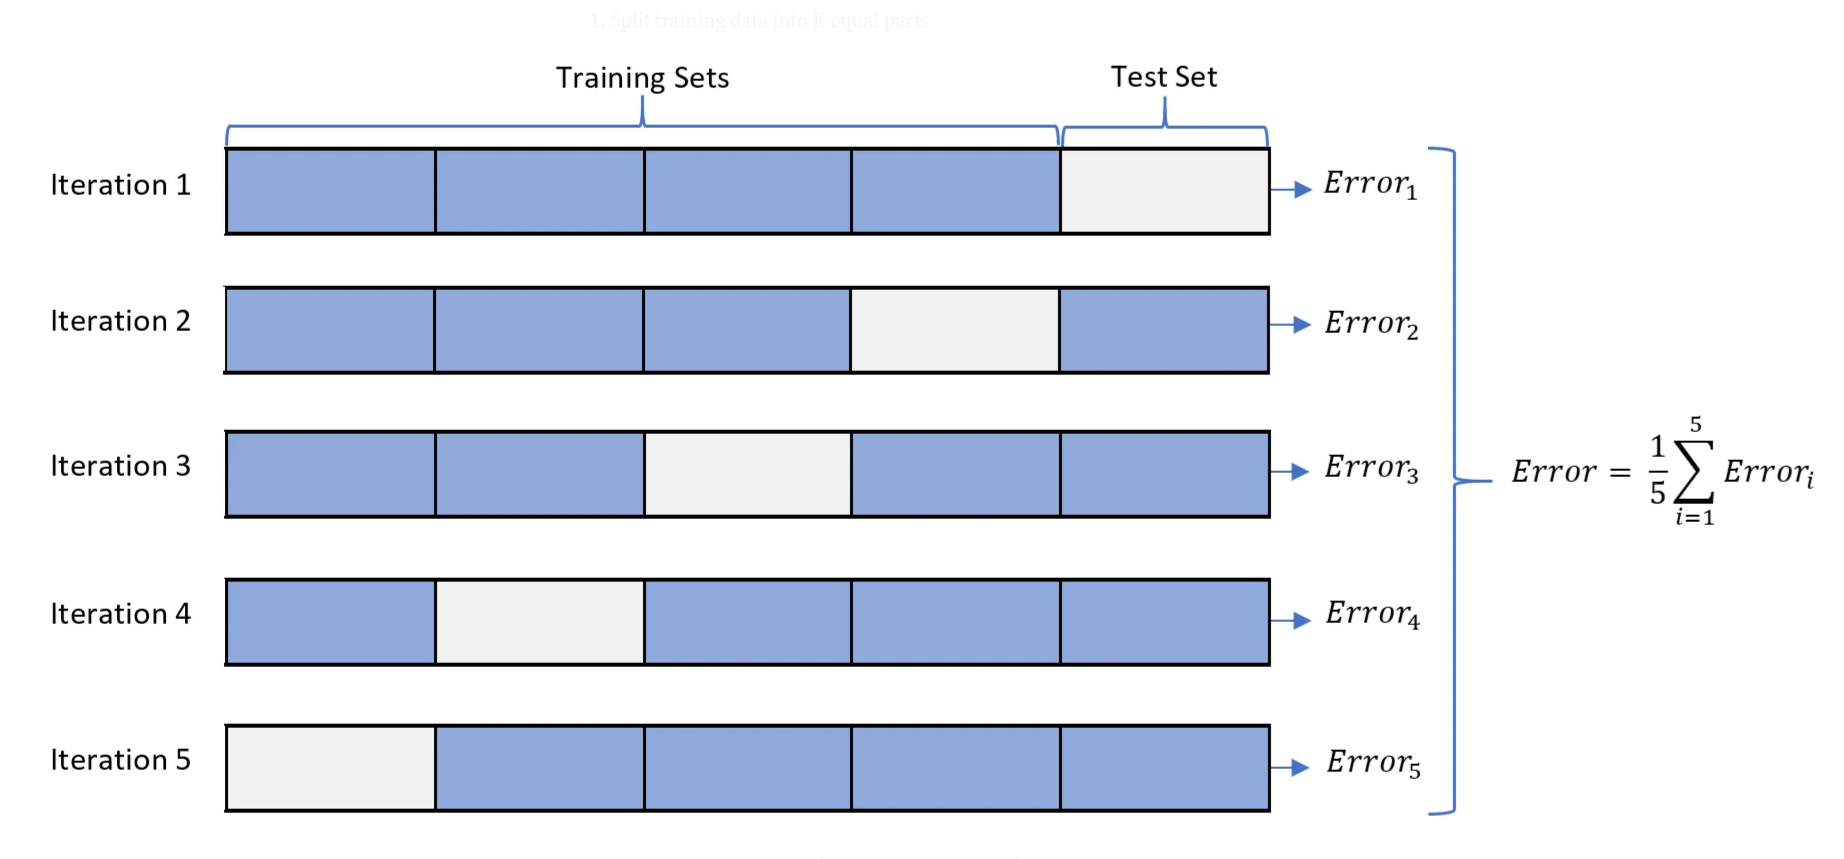
\includegraphics[width=0.9\textwidth]{informatica/kfold_cross_val_img_example}
    \caption{Ejemplo gráfico del uso de \textit{K-Fold Cross Validation}, con un valor de $K = 5$. Cada fila representa una iteración del proceso. Las partes azules representan los 4 \textit{folds} elegidos en esa iteración para entrenar. La parte blanca representa el \textit{fold} que usamos para calcular la métrica a optimizar. Imagen extraída de \cite{informatica:kfold_cross_val_img_web}}
    \label{img:visualizacion_kfold_cv}
\end{figure}

Tenemos que tener en cuenta una serie de cuestiones a la hora de aplicar esta técnica:

\begin{itemize}
    \item Cuanto mayor sea el valor de $K$ mejor. De esta forma, reducimos la variabilidad que supone elegir determinados \textit{folds} para validar, y la métrica obtenida al final como un promedio es más robusta
    \item De hecho, cuando tomamos $K$ igual al número de elementos del \textit{dataset}, estamos aplicando la técnica conocida como \textit{leave-one-out} \cite{informatica:kfold_cross_val_paper}
    \item Sin embargo, valores altos de $K$ suponen tiempos de cómputo grandes: entrenamos $K$ veces, y sobre un porcentaje grande del \textit{dataset} de entrenamiento: $\frac{K - 1}{K}$
\end{itemize}

Describimos cómo implementamos estas dos técnicas (\textit{holdout} y \textit{K-fold Cross validation}) en \sectionref{isec:hp_tuning}.

\subsection{Normalización} \label{isubs:normalizacion_teoria}

En \sectionref{isec:triplet_loss} hemos comentado el problema que puede suponer que la red aprenda a colapsar cualquier entrada al vector $\vec{0}$. Aunque añadimos un margen $\alpha$ para evitar este comportamiento, en \sectionref{isec:margenes_suaves} introducimos una variante en la que podría llegar a aprenderse este mal comportamiento. Por tanto, otra técnica a explorar es la de normalizar las salidas de la red, forzando a que tengan norma unitaria. Esta técnica se usa en \cite{informatica:facenet}. La normalización consiste en realizar la siguiente sustitución:

\begin{equation} \label{ieq:normalizacion}
    \hat{x} := \frac{f_{\theta}(x)}{||f_{\theta}(x)||_2}
\end{equation}

Además del interés que pueda tener estudiar el comportamiento de los modelos al introducir la normalización, esta técnica introduce el siguiente punto a tener en cuenta. Durante los entrenamientos hemos tenido muchos problemas de inestabilidad:  en la mayoría de ocasiones, el entrenamiento se saturaba tras pocas iteraciones. Es claro que si nuestra red aprende a colapsar todas las entradas a $\vec{0}$, la ecuación \eqref{ieq:normalizacion} falla, con lo que el entrenamiento se detiene. Sin embargo, a raíz de la experimentación, vemos que la normalización ayuda enormemente a que dicho comportamiento no se aprenda. Y con ello, es mucho más fácil conseguir entrenamientos estables. El siguiente diagrama muestra un ejemplo de entrenamiento inestable:

\begin{figure}[H]
    \centering
    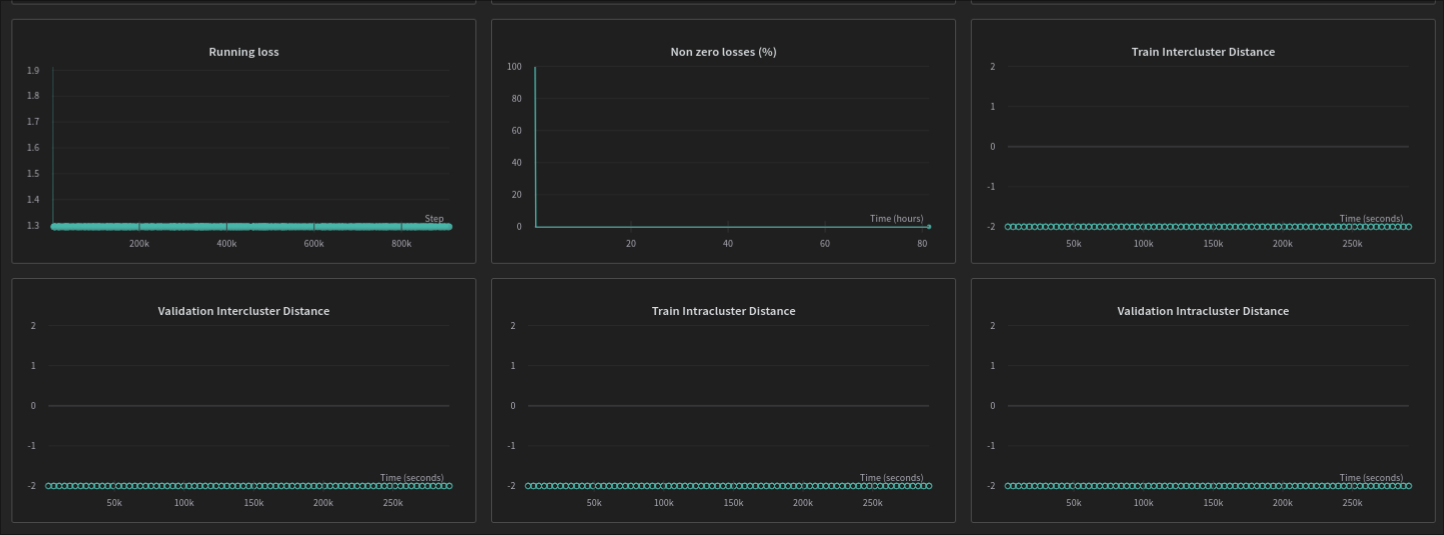
\includegraphics[width=0.8\textwidth]{informatica/ejemplo_colapso_entrenamiento}
    \caption{Histórico de \textit{WANDB} que muestra un entrenamiento inestable que acaba por fallar. En las gráficas, los círculos indican entradas con el valor \lstinline{NaN}}
\end{figure}

En \sectionref{isubs:normalization_impl} estudiaremos la implementación de esta técnica en detalle.

\subsection{Localización de cuellos de botella en el código para realizar optimizaciones} \label{isubs:localizacion_partes_criticas}

Como hemos comentado en \sectionref{isec:planificacion} y \sectionref{isec:base_datos_usada}, hemos iterado sobre distintas bases de datos, aumentando la complejidad y tamaño de estas sin preocuparnos demasiado sobre la eficiencia de nuestras implementaciones, hasta que hemos encontrado problemas considerables debidos a los tiempos de ejecución. Una vez que nos encontramos con estos problemas, identificamos qué partes del código son las responsables. Llamamos \textbf{cuellos de botella} o \textit{bottlenecks} a estas partes de código responsables de tiempos de ejecución elevados

Realizaremos un \textit{profile} para identificar los cuellos de botella (véase \sectionref{isec:optimizacion_codigo}). Una vez identificamos \textit{bottlenecks}, sabemos en qué partes concretas debemos concentrar nuestros esfuerzos. De esta forma desarrollamos una amplia base de código inicial de forma rápida, sin aplicar optimizaciones prematuras. Y las optimizaciones que realizamos son óptimas, pues estamos localizando el código responsable de los tiempos de cómputo.

El enfoque que acabamos de describir se fundamenta en la \textbf{ley de Amdahl} \cite{informatica:amdahl_original} \cite{informatica:amdahl_moderno}. Aunque esta ley se centra en medir mejoras de tiempo al introducir paralelismo, es fácilmente aplicable a nuestro ámbito: cambios en las implementaciones para acelerar los tiempos de cómputo. Si optimizamos una fracción de cómputo $f$ obteniendo una mejora en tiempo de cómputo de $S$ para esa fracción, la mejora global (mejora que obtenemos sobre toda la base de código) viene dada por:

\begin{equation} \label{eq:amdahl}
    S_{global} := \frac{1}{(1 - f) + \frac{f}{S}}
\end{equation}

Además, suponiendo que optimicemos infinitamente la fracción de cómputo, hasta tal punto que sea instantánea de computar, la mejora estaría limitada de la siguiente forma:

\begin{equation}
    S_{max} := \lim_{S \to \infty}\frac{1}{(1 - f) + \frac{f}{S}} = \frac{1}{1 - f}
\end{equation}

Por tanto, aunque una mejora de cómputo sea muy buena, si se realiza sobre una porción de código con un valor de $f$ bajo, el impacto no será relevante. Es decir, no debemos fijarnos únicamente en lo buena que sea una optimización, sino que también debemos encontrar aquellas partes del código que mayor tiempo de cómputo (mayor valor de $f$) estén suponiendo. Esto justifica el enfoque que empleamos en \sectionref{isec:optimizacion_codigo}.

\section{Mejoras técnicas objeto de estudio} \label{isec:mejoras_tecnicas_objeto_de_estudio}

Hemos introducido todos los conceptos teóricos suficientes para plantear una solución basada en aprendizaje automático para nuestro problema. Sin embargo, una \textbf{parte fundamental de este trabajo consiste en explorar algunas mejoras técnicas} introducidas en \cite{informatica:principal}. Dichas mejoras se resumen en:

\begin{itemize}
    \item Introducir una técnica para minar de forma \textit{online} los triples, basada en el muestreo \textit{PK-Sampling}
    \item A partir del nuevo muestreo podemos definir dos variaciones sobre la función de pérdida
    \item Exploramos el uso de una nueva función de distancia
\end{itemize}

\subsection{Enfoque online de \textit{Triplet Loss}} \label{isubs:triples_online}

Buscamos modificar el minado de triples \textit{offline} para solucionar alguno de sus problemas que hemos comentado. Para ello implementaremos el siguiente proceso. En primer lugar, realizaremos un muestreo aleatorio sobre nuestros datos de la forma \lstinline{(imagen, identidad, edad)}. Este muestreo es rápido y no supone prácticamente tiempo de cómputo. Usando únicamente los datos de ese muestreo, generaremos triples y computaremos la función de pérdida apoyándonos en \eqref{ieq:triplet_loss_single_entry}. Dicha generación ya sí que supone un tiempo de cómputo considerable. Repetimos este proceso hasta agotar todos las entradas de nuestro \textit{dataset}, completando así una época de entrenamiento.

Ya podemos ver algunas \textbf{ventajas de este método}, incluso antes de haber especificado las dos partes fundamentales del proceso (muestreo y selección de triples):

\begin{enumerate}
    \item La ventaja más obvia es que, suponiendo que el tamaño de la muestra es significativamente mucho más pequeño que el tamaño de todo el conjunto de datos, la generación de triples consumirá potencialmente menos tiempo y será más efectiva
        \begin{itemize}
            \item Para afirmar esto rotundamente, tendríamos que realizar un estudio del tiempo del minado \textit{offline} en contraste a la suma de todos los tiempos de minado en cada muestreo
            \item Sin embargo, el tiempo usado es más eficiente, porque en cada muestreo estamos usando la red actualizada. En el minado \textit{offline} podemos gastar muchísimo tiempo en encontrar triples difíciles que, tras entrenar en unos pocos triples previos, acaben siendo sencillos. Por tanto, cuando la red vea triples algo avanzados en la lista, estos ya serán totalmente inútiles
        \end{itemize}
    \item Se facilita en gran parte el ajuste de la dificultad. Podemos buscar triples realmente difíciles, pero como solo se tiene acceso a una pequeña muestra, estamos controlando la dificultad. Así que podemos variar el tamaño de las muestras para buscar un punto medio entre ejemplos muy difíciles o ejemplos demasiado sencillos. Y todo esto sin contar con el factor de que vamos a usar la red actualizada para la elección de los triples
\end{enumerate}

Desarrollada esta visión de forma general, veamos cómo se implementa cada una de las partes, siguiendo las técnicas introducidas en \cite{informatica:principal}.

\subsection{Generación online de \textit{batches} usando \textit{P-K sampling}} \label{isubs:muestreo_datos_pk_sampling_teoria}

La \textbf{idea principal del muestreo} es lo que definiremos como \textbf{\textit{P-K sampling}}. Como ya hemos comentado en \sectionref{isubs:triples_online}, nuestra tarea ahora es generar un \textit{batch} de elementos de la forma \lstinline{(imagen, identidad, edad)}. En una segunda etapa (véase \sectionref{isubs:seleccion_de_triples}), otro algoritmo decide cómo generar triples a partir de estos datos.

El algoritmo de muestreo \textit{P-K sampling} es muy sencillo. En cada muestreo, seleccionamos aleatoriamente $P$ identidades de individuos (o clases, en un ambiente más general en el que no necesariamente estemos trabajando con imágenes de personas). Por cada una de las identidades, seleccionamos aleatoriamente $K$ imágenes asociadas a esa identidad. Por tanto, obtenemos una lista de $P \cdot K$ imágenes, a la que llamaremos \textbf{\textit{P-K batch}}. Para poder obtener triples interesantes en la siguiente etapa, parece que lo deseable es que ambos muestreos aleatorios sean sin repetición.

El hecho de tener $K$ imágenes por cada uno de los individuos seleccionados es lo que va a permitir al algoritmo de generación de triples obtener rápidamente triples interesantes.

\begin{figure}[H]
    \centering
    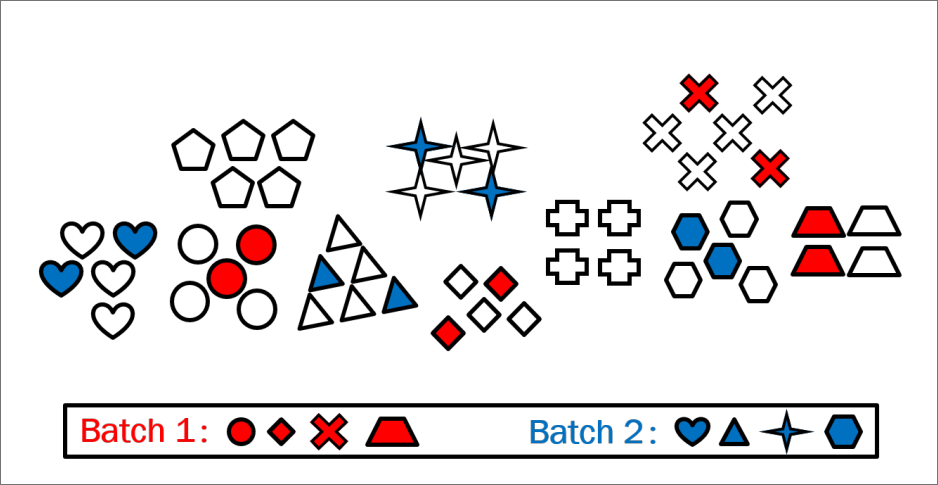
\includegraphics[width=0.6\textwidth]{informatica/ejemplo_grafico_pk_sampling}
    \caption{Ejemplo gráfico del proceso de \textit{P-K sampling}. Imagen extraída de \cite{informatica:paper_image_pk_sampling}}
\end{figure}

Queda aquí claro el \textbf{problema principal} que introduce esta técnica: si queremos muestrear $K$ imágenes de cada individuo sin repetición, cada individuo debe tener asociadas al menos $K$ imágenes. Así que a la hora de trabajar con un \textit{dataset}, siempre deberíamos comprobar la distribución del número de imágenes por individuo, como haremos en \sectionref{isec:base_datos_usada}.

\subsection{Selección de triples y variaciones en la función de pérdida} \label{isubs:seleccion_de_triples}

Una vez que tenemos un \textit{batch} de $P \cdot K$ elementos, deberemos generar una lista de triples en base a este \textit{batch}. Una vez se especifica cómo se seleccionan los triples, usando \eqref{ieq:triplet_loss_single_entry}, inducimos de forma natural y directa una cierta función de pérdida que actúa sobre estos \textit{P-K batches}.

Introducimos una notación que nos va a ser útil. Trabajamos $P \cdot K$ elementos, cada uno correspondiendo a una clase en concreto. Por tanto, indexaremos los elementos de la forma $x_k^p$ donde $p$ marca el identificador del individuo, y $k$ marca a cuál de las $K$ imágenes del individuo $p$ nos estamos refiriendo

\subsubsection{\textit{Batch Hard}} \label{isubsubs:batch_hard}

La primera idea es iterar sobre todos los elementos del \textit{P-K batch}, obteniendo así $P \cdot K$ anclas. Por cada ancla, seleccionamos el positivo y negativo \textbf{más complicado dentro de \textit{P-K batch}}. Por tanto, queda claro que \textbf{estamos usando la red para seleccionar triples difíciles} en cada \textit{batch} generado.

Esto introduce la siguiente función de pérdida, a la que llamaremos \textbf{\textit{Batch Hard}}:

\begin{equation}
    \mathcal{L}_{BH}(\theta, \hat{\Omega}) := \comentarencima{\sum_{p = 1}^P \sum_{k = 1}^K}{\text{todas las anclas}} [
        \comentarencima{\max_{k' = 1, \ldots, K} D(f_{\theta}(x_k^p), f_{\theta}(x_{k'}^p))}{\text{positivo más complicado}}
        - \comentarencima{\min_{\substack{p' = 1, \ldots, P \\ p' \neq p \\ k' = 1, \ldots, K}} D(f_{\theta}(x_k^p), f_{\theta}(x_{k'}^{p'}))}{\text{negativo más complicado}}
        + \alpha]_+
\end{equation}

donde $[x]_+ := max \{0, x\} = ReLU(x)$ y $\hat{\Omega}$ se refiere a un \textit{P-K batch}. No olvidemos que no estamos escribiendo la división por el número de sumandos, $P \cdot K$.

Estamos generando \textbf{triples moderados}, porque estamos buscando los triples más difíciles, pero dentro de un \textit{batch} relativamente pequeño comparado a el total del conjunto de datos. Con esto estamos ajustando la dificultad de los triples cómodamente, resolviendo el problema que comentábamos en \sectionref{isubs:enfoque_offline_minado_triples}. Aumentando el valor de $\{P, K\}$ aumentamos el tamaño del espacio de búsqueda, y por tanto podremos encontrar triples mucho más difíciles. Sin embargo, hay que tener siempre en cuenta el coste en tiempo de cómputo.

Queda claro que, gracias al proceso de \textit{P-K sampling}, ahora es factible realizar una búsqueda de triples interesantes en profundidad, basándonos en el estado más actualizado de la red para calcular la dificultad de los triples. Esta búsqueda extensiva no habría sido posible si la planteásemos sobre todo el conjunto de datos.

\subsubsection{\textit{Batch All}} \label{isubsubs:batch_all}

Motivados por lo que acabamos de comentar en \sectionref{isubsubs:batch_hard}, podemos plantearnos usar todos los posibles triples dentro de un \textit{P-K batch} como un enfoque que ahora cobra más sentido (ya hemos comentado en \sectionref{isubs:enfoque_offline_minado_triples} que realizar esto sobre todo el conjunto de datos no parece una buena idea).

Realizar esto introduce la función de pérdida que llamaremos \textbf{\textit{Batch All}}:

\begin{equation} \label{ieq:batch_all}
    \mathcal{L}_{BA}(\theta; \hat{\Omega}) :=
    \comentarencima{\sum_{p = 1}^{P} \sum_{k = 1}^K}{\text{todas anclas}}
    \comentardebajo{\sum_{\substack{k' = 1 \\ k' \neq k}}^{K}}{\text{todas pos.}}
    \comentarencima{\sum_{\substack{p' = 1 \\ p' \neq p}}^P \sum_{n = 1}^K}{\text{todas neg.}} \dspace[
        D(f_{\theta}(x_k^p),f_{\theta}(x_{k'}^p)) - D(f_{\theta}(x_k^p),f_{\theta}(x_{n}^{p'})) + \alpha
    ]_+
\end{equation}

Está claro que, por el número de sumandos, esta aproximación es viable gracias a que nuestro \textit{P-K sampling} reduce mucho el número de elementos sobre los que operamos. Dicho número de sumandos viene dado por:

\begin{equation}
    P \cdot K \cdot (K - 1) \cdot (P - 1) \cdot K = P^2 - P + K^3 - K^2 \approx P^2 + K^3
\end{equation}

Esta aproximación sería completamente inviable sobre un número muy elevado de elementos. Pensemos, por ejemplo, en las 163446 imágenes de \textit{CACD} (conjunto de datos que estudiamos en \sectionref{isec:dataset_cacd}).

\subsubsection{Mejoras introducidas a partir de la experimentación} \label{isubsubs:mejoras_sumandos_no_nulos}

En \cite{informatica:principal}, a raíz de observar los resultados de la experimentación, señalan algunos puntos débiles en las dos funciones de pérdida que introducen a partir del \textit{P-K sampling}.

Principalmente, en \customref{isubsubs:batch_all}, podemos ver un posible fallo en la función de pérdida \eqref{ieq:batch_all}. Si se da el caso de que la mayoría de triples generados son fáciles (hecho muy probable al estar generando todas las combinaciones de triples), los escasos triples que realmente son difíciles se desvanecerán. Esto porque la mayoría de términos serán cero (al estar aplicando $[x]_+$). Y los pocos términos que no son cero, se dividen por el número total de elementos, que ya hemos visto que es elevado.

Por tanto, una mejora sencilla a esta función de pérdida es dividir únicamente por el número de sumandos no nulos. A estos sumandos no nulos también se les llama sumandos activos \cite{informatica:principal}. Esta mejora la podemos aplicar también a \textit{batch hard}, obteniendo dos nuevas funciones de pérdida, a las que denotaremos por $\mathcal{L}_{BA \neq 0}$ y $\mathcal{L}_{BH \neq 0}$.

\subsubsection{Algunas observaciones y conclusiones} \label{isubsubs:observaciones_conclusiones_pksampling}

En primer lugar, cabe destacar que, como señalan \cite{informatica:principal}, las dos nuevas funciones de pérdida introducidas equivalen al planteamiento clásico de \textit{triplet loss} si entrenásemos indefinidamente.

El desarrollo que hemos realizado justifica las siguientes \textbf{ventajas} de los nuevos métodos:

\begin{itemize}
    \item El uso del \textit{P-K sampling} y las dos nuevas funciones de pérdida (con las variantes técnicas que consideran los sumandos activos) permite realizar un aprendizaje \textit{end-to-end}, sin añadir un paso adicional en el bucle de aprendizaje, evitando así la gran complejidad añadida del minado \textit{offline}
    \item Además, conseguimos un manejo preciso de la dificultad de los triples obtenidos. Controlando el valor de $\{P, K\}$, controlamos el espacio de búsqueda y, en definitiva, la dificultad. Todo esto de forma cómoda y sin introducir apenas complejidad en nuestro \textit{pipeline}
    \item Aunque no lo hemos comprobado, pensamos que esto acelera los tiempos de cómputo, al estar realizando el minado de triples sobre \textit{batches} de tamaño considerablemente reducidos
    \item Y aunque no mejorásemos el tiempo de computo, lo que sí sabemos que mejoramos es la eficacia del minado de triples. El minado de triples \textit{online} usa una red mucho más actualizada, para generar una lista mucho más pequeña que probablemente no se degrade tanto como la generada por un minado \textit{offline} sobre todo el conjunto de datos, mucho más grande
    \item Es más, estamos controlando el efecto de los triples demasiado sencillos, que no tendremos en cuenta a la hora de promediar en la función de pérdida
\end{itemize}

A pesar de esto, a raíz de trabajar con estas nuevas técnicas, identificamos los siguientes \textbf{inconvenientes}:

\begin{itemize}
    \item Introducimos dos hiperparámetros, $\{P, K\}$ que deberemos ajustar correctamente, pues tienen un enorme impacto en los resultados del proceso de entrenamiento. Por tanto, se hace fundamental tener un proceso de \textit{hyperparameter tuning} robusto, como introducimos en \sectionref{isec:hptuning_kfold_cross_validation} e implementamos en \sectionref{isec:hp_tuning}
    \item Tenemos que tener mucho cuidado con usar valores elevados de $\{P, K\}$ por dos motivos. El primero, y como ya hemos comentado, valores altos implicarán que los tiempos de cómputo para la generación de triples crecerán rápidamente. El segundo es que el tamaño de los \textit{batches} crecerán considerablemente, llegando a colapsar la memoria disponible de la \textit{GPU}
    \item Hemos comprobado en la práctica que es realmente fácil colapsar la memoria \textit{GPU}, usando modelos profundos como \textit{ResNet50} con valores de $P \cdot K = 100$. Esto supone que, aunque no estuviéramos limitados por el tiempo de cómputo, el colapso de la memoria limita el conjunto de valores $\{P, K\}$ con los que podemos experimentar
    \item Si queremos usar valores altos de $K$, nuestro \textit{dataset} lo debe permitir, teniendo una buena distribución de imágenes por individuo. Por este motivo hemos estudiado esta distribución en \sectionref{isec:base_datos_usada}. Se pueden explorar técnicas como el aumentado de datos para alcanzar el número de imágenes por individuo deseado, pero solo serán efectivas si dicha distribución es buena para empezar (véase \sectionref{isec:aumentado_datos})
    \item Tanto por el formato de los datos con los que hemos trabajado, como por el cambio fundamental realizado en el \textit{sampling} de los datos, hemos tenido que realizar un \textbf{esfuerzo considerable de implementación}, al no poder basarnos en la mayor parte de los casos en código implementado por alguna biblioteca de aprendizaje automático. Esto se ve reflejado en \sectionref{ich:implementacion}
\end{itemize}

\subsection{Variaciones en la función de distancia}

En todos los conceptos que hemos ido introduciendo la función de distancia

\begin{equation}
    D: X \times X \to [0, \infty)
\end{equation}

ha estado presente, pero todavía no hemos introducido ninguna función concreta. En el ambiente de \textit{AIFR} se suele usar la distancia euclídea al cuadrado, esto es:

\begin{equation}
    D(x_i, x_j) := ||f_{\theta}(x_i) - f_{\theta}(x_j)||^2_2
\end{equation}

Sin embargo, motivados por \cite{informatica:principal}, decidimos usar la distancia euclídea usual. En este trabajo se afirma que, en base a la experimentación, de esta forma se obtienen entrenamientos más estables. Además, usando la distancia euclídea usual, el margen es más fácil de interpretar, porque marca la diferencia de distancias, y no la diferencia de cuadrados de distancias. Por lo tanto, en base a dicho trabajo, decidimos tomar:

\begin{equation}
        D(x_i, x_j) := ||f_{\theta}(x_i) - f_{\theta}(x_j)||_2
\end{equation}

\subsection{Márgenes suaves} \label{isec:margenes_suaves}

En \sectionref{isec:triplet_loss} hemos justificado por qué es necesario introducir un término $\alpha$ para controlar el margen y evitar que nuestro modelo aprenda a colapsar todas las entradas al vector $\vec{0}$. Con esto llegamos a la ecuación \eqref{ieq:triplet_loss_single_entry}.

En dicha función de pérdida, el propósito de $x \mapsto \max\{0, x + \alpha\}$ (conocida comúnmente como \textit{hinge function}) es no corregir ejemplos que, en vista del margen $\alpha$ establecido, ya son correctos. Pero puede ser que estemos interesados en afinar aún más ejemplos que, para dicho valor del margen, sean correctos. Con esto conseguiríamos seguir acercando imágenes del mismo individuo lo máximo posible \cite{informatica:principal}. Es por esto que se propone en usar la función \textbf{\textit{softplus}}:

\begin{equation}
    x \mapsto ln(1 + exp(x))
\end{equation}

Dicha función puede verse como una versión suavizada de la función \textit{hinge}. Decae exponencialmente, por lo que ejemplos correctos se penalizarán exponencialmente menos cuanto más cercanos estén, pero contrasta con la función \textit{hinge} en que no presenta un salto o corte fuerte. Por tanto, se suele decir que estamos usando un \textbf{margen suave}. Además, una ventaja de esta función es que \textbf{desechamos el hiperparámetro $\alpha$}, el cual ya no tenemos que fijar a través de algún método (como podría ser el \textit{hyperparameter tuning}).

\begin{figure}[H]
\centering
    \begin{subfigure}{.5\textwidth}
        \centering
        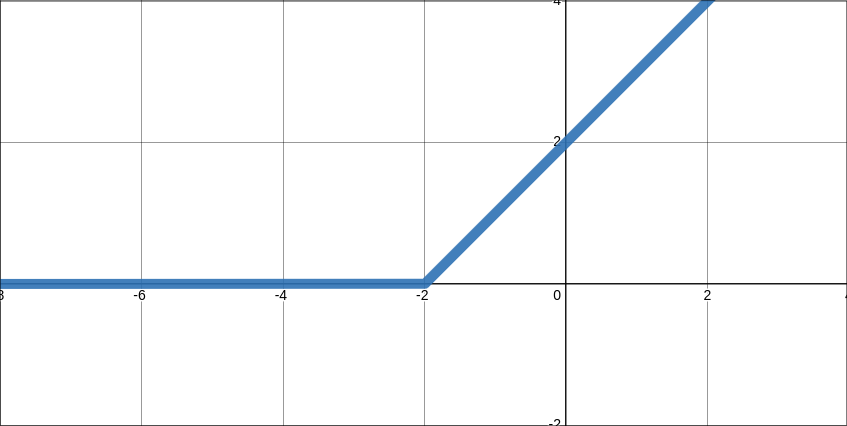
\includegraphics[width=0.8\linewidth]{informatica/desmos_hinge}
        \caption{Función \textit{hinge} con $\alpha = 2$}
    \end{subfigure}%
    \begin{subfigure}{.5\textwidth}
        \centering
        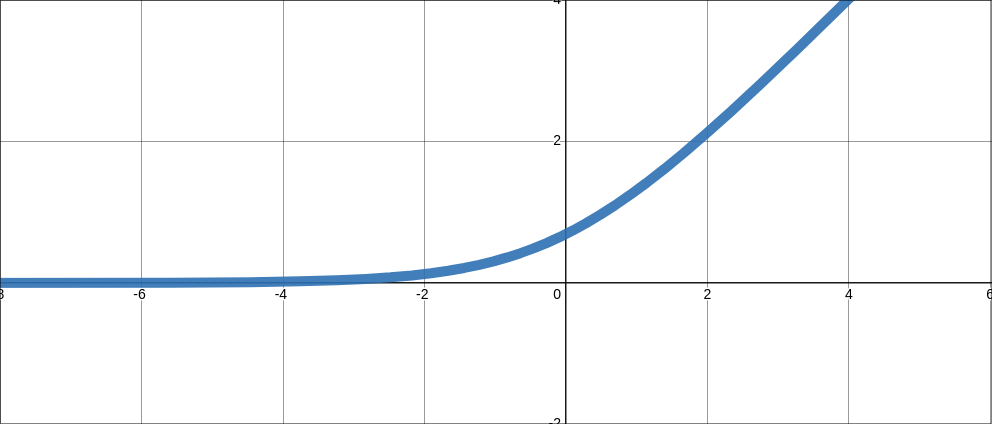
\includegraphics[width=0.8\linewidth]{informatica/desmos_softplus}
        \caption{Función \textit{softplus}}
    \end{subfigure}

    \begin{subfigure}{.5\textwidth}
        \centering
        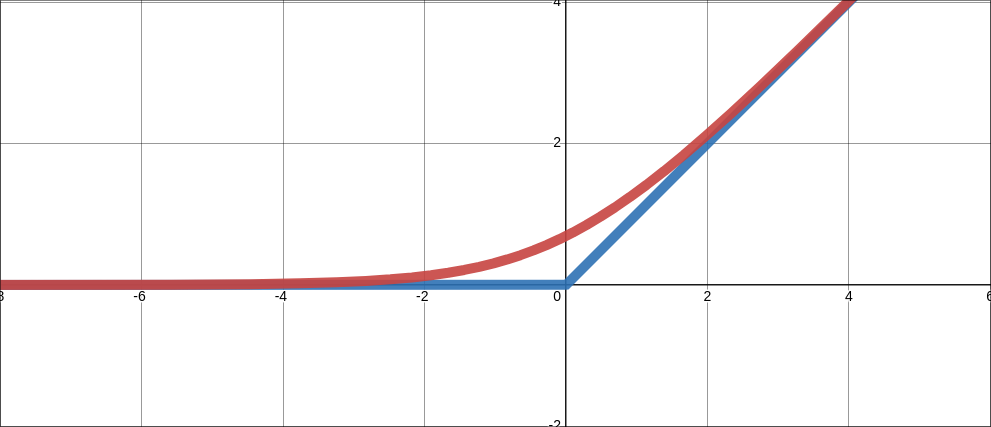
\includegraphics[width=0.8\linewidth]{informatica/desmos_conjunta}
        \caption{En azul, \textit{hinge} con $alpha = 0$. En rojo, \textit{softplus}}
    \end{subfigure}


\caption{Gráfica de las dos funciones para trabajar con los márgenes, y una gráfica conjunta que muestra su similitud}
    \label{img:graficas_margenes}
\end{figure}

Las gráficas mostradas en \imgref{img:graficas_margenes} nos sirven para visualizar de forma sencilla todo lo que hemos comentado. La función \textit{softplus} actúa como una \textit{hinge} suavizada. El hecho de que se parezcan tanto cuando hacemos que el margen de \textit{hinge} sea cero nos hace pensar que \textit{softplus} va a actuar como una \textit{hinge} en la que no hay margen, y por lo tanto, acercará elementos de la misma clase todo lo que pueda.
